\def\year{2021}\relax
%File: formatting-instructions-latex-2021.tex
%release 2021.2
\documentclass[letterpaper]{article} % DO NOT CHANGE THIS

\usepackage{aaai21_no_copyright}  % DO NOT CHANGE THIS
\usepackage{soul}
\usepackage{times}  % DO NOT CHANGE THIS
\usepackage{helvet} % DO NOT CHANGE THIS
\usepackage{courier}  % DO NOT CHANGE THIS
\usepackage[hyphens]{url}  % DO NOT CHANGE THIS
\usepackage{graphicx} % DO NOT CHANGE THIS
\urlstyle{rm} % DO NOT CHANGE THIS
\def\UrlFont{\rm}  % DO NOT CHANGE THIS
\usepackage{natbib}  % DO NOT CHANGE THIS AND DO NOT ADD ANY OPTIONS TO IT
\usepackage{caption} % DO NOT CHANGE THIS AND DO NOT ADD ANY OPTIONS TO IT
\frenchspacing  % DO NOT CHANGE THIS
\setlength{\pdfpagewidth}{8.5in}  % DO NOT CHANGE THIS
\setlength{\pdfpageheight}{11in}  % DO NOT CHANGE THIS
%\nocopyright
%PDF Info Is REQUIRED.
% For /Author, add all authors within the parentheses, separated by commas. No accents or commands.
% For /Title, add Title in Mixed Case. No accents or commands. Retain the parentheses.
\pdfinfo{
/Title (PLGRIM: Hierarchical Value Learning for Large-scale Autonomous Exploration in Unknown Environments)
/Author (Sung-Kyun Kim*, Amanda Bouman*, Gautam Salhotra, David D. Fan, Kyohei Otsu, Joel Burdick, Ali-akbar Agha-mohammadi)
/TemplateVersion (2021.2)
} %Leave this

% DISALLOWED PACKAGES
% \usepackage{authblk} -- This package is specifically forbidden
% \usepackage{balance} -- This package is specifically forbidden
% \usepackage{color (if used in text)
% \usepackage{CJK} -- This package is specifically forbidden
% \usepackage{float} -- This package is specifically forbidden
% \usepackage{flushend} -- This package is specifically forbidden
% \usepackage{fontenc} -- This package is specifically forbidden
% \usepackage{fullpage} -- This package is specifically forbidden
% \usepackage{geometry} -- This package is specifically forbidden
% \usepackage{grffile} -- This package is specifically forbidden
% \usepackage{hyperref} -- This package is specifically forbidden
% \usepackage{navigator} -- This package is specifically forbidden
% (or any other package that embeds links such as navigator or hyperref)
% \indentfirst} -- This package is specifically forbidden
% \layout} -- This package is specifically forbidden
% \multicol} -- This package is specifically forbidden
% \nameref} -- This package is specifically forbidden
% \usepackage{savetrees} -- This package is specifically forbidden
% \usepackage{setspace} -- This package is specifically forbidden
% \usepackage{stfloats} -- This package is specifically forbidden
% \usepackage{tabu} -- This package is specifically forbidden
% \usepackage{titlesec} -- This package is specifically forbidden
% \usepackage{tocbibind} -- This package is specifically forbidden
% \usepackage{ulem} -- This package is specifically forbidden
% \usepackage{wrapfig} -- This package is specifically forbidden
% DISALLOWED COMMANDS
% \nocopyright -- Your paper will not be published if you use this command
% \addtolength -- This command may not be used
% \balance -- This command may not be used
% \baselinestretch -- Your paper will not be published if you use this command
% \clearpage -- No page breaks of any kind may be used for the final version of your paper
% \columnsep -- This command may not be used
% \newpage -- No page breaks of any kind may be used for the final version of your paper
% \pagebreak -- No page breaks of any kind may be used for the final version of your paperr
% \pagestyle -- This command may not be used
% \tiny -- This is not an acceptable font size.
% \vspace{- -- No negative value may be used in proximity of a caption, figure, table, section, subsection, subsubsection, or reference
% \vskip{- -- No negative value may be used to alter spacing above or below a caption, figure, table, section, subsection, subsubsection, or reference

% \setcounter{secnumdepth}{0} %May be changed to 1 or 2 if section numbers are desired.
\setcounter{secnumdepth}{2} %May be changed to 1 or 2 if section numbers are desired.


\graphicspath{{../}{./}{./figures/}}


%%%%%%%%%%%%%%%%%%%%%%%%%%%%%%%%%%%%%%%
%%%%%%%%%%%%%%%%%%%%%%%%%%%%%%%%%%%%%%%

\usepackage[utf8]{inputenc}
\usepackage[T1]{fontenc}
\usepackage{graphicx}
\usepackage{float}
\usepackage{xcolor}
\usepackage[normalem]{ulem}
\usepackage{subfig}

\usepackage{amsmath}
\usepackage{amsfonts}
\usepackage{amssymb}
\usepackage{mathtools}
\usepackage{todonotes}
\usepackage{enumitem}
\usepackage{multicol}
\usepackage{comment}
% \usepackage[noend]{algpseudocode} % this breaks my algorithm box

\usepackage{tikzpagenodes}

% \usepackage[
%   subtle
%   %moderate
% ]{savetrees}

\usepackage{algorithm,algorithmic}

\newcommand{\ph}[1]{{\textbf{#1}:}} % paragraph header
% \newcommand{\phdone}[1]{{\textbf{#1}:}} % (invisible) paragraph header
\newcommand{\phdone}[1]{} % (invisible) paragraph header
\newcommand{\ncomment}[1]{}
\newcommand{\acomm}[1]{{\color{cyan}Ali:#1}} % Ali's comments from video
% \newcommand{\todo}[1]{{\color{red} #1 }} % Tasks to do
\newcommand{\note}[1]{{\color{red}#1 }}
\newcommand{\maximize}{\mathop{\mathrm{maximize}}}
\newcommand{\argmax}{\mathop{\mathrm{argmax}}}
\newcommand{\argmin}{\mathop{\mathrm{argmin}}}

%%%%%%%%%%%%%%%%%%%%%%%%%%%%%%%%%%%%%%%
%%%%%%%%%%%%%%%%%%%%%%%%%%%%%%%%%%%%%%%



% The file aaai21.sty is the style file for AAAI Press
% proceedings, working notes, and technical reports.
%

% Title

% Your title must be in mixed case, not sentence case.
% That means all verbs (including short verbs like be, is, using,and go),
% nouns, adverbs, adjectives should be capitalized, including both words in hyphenated terms, while
% articles, conjunctions, and prepositions are lower case unless they
% directly follow a colon or long dash

\title{
    PLGRIM: Hierarchical Value Learning for \\Large-scale Autonomous Exploration in Unknown Environments
}
\author{
		Sung-Kyun Kim,\thanks{These authors contributed equally to this work. \newline \hspace*{1.1em} \copyright2020. All rights reserved.}\textsuperscript{\rm 1}
    Amanda Bouman,$^{*}$\textsuperscript{\rm 2}
    Gautam Salhotra,\textsuperscript{\rm 3}
    David D. Fan,\textsuperscript{\rm 1} \\
    Kyohei Otsu,\textsuperscript{\rm 1}
    Joel Burdick,\textsuperscript{\rm 2}
    Ali-akbar Agha-mohammadi\textsuperscript{\rm 1} \\
}
\affiliations{
    \textsuperscript{\rm 1}
    NASA Jet Propulsion Laboratory,
    California Institute of Technology
    \\ \{sung.kim,
    david.d.fan,
    kyohei.otsu,
    aliagha\}\!@jpl.nasa.gov
    % \\ aliakbar.aghamohammadi@jpl.nasa.gov
    \\
    \textsuperscript{\rm 2}
    Department of Mechanical and Civil Engineering,
    California Institute of Technology
    \\ abouman@caltech.edu,
    jwb@robotics.caltech.edu
    \\
    \textsuperscript{\rm 3}
    Department of Computer Science,
    University of Southern California
    \\ salhotra@usc.edu
}
% \author{
%     %Authors
%     % All authors must be in the same font size and format.
%     Written by AAAI Press Staff\textsuperscript{\rm 1}\thanks{With help from the AAAI Publications Committee.}\\
%     AAAI Style Contributions by Pater Patel Schneider,
%     Sunil Issar,  \\
%     J. Scott Penberthy,
%     George Ferguson,
%     Hans Guesgen,
%     Francisco Cruz,
%     Marc Pujol-Gonzalez
%     \\
% }
% \affiliations{
%     %Afiliations
%     \textsuperscript{\rm 1}Association for the Advancement of Artificial Intelligence\\
%     %If you have multiple authors and multiple affiliations
%     % use superscripts in text and roman font to identify them.
%     %For example,
%
%     % Sunil Issar, \textsuperscript{\rm 2}
%     % J. Scott Penberthy, \textsuperscript{\rm 3}
%     % George Ferguson,\textsuperscript{\rm 4}
%     % Hans Guesgen, \textsuperscript{\rm 5}.
%     % Note that the comma should be placed BEFORE the superscript for optimum readability
%
%     2275 East Bayshore Road, Suite 160\\
%     Palo Alto, California 94303\\
%     % email address must be in roman text type, not monospace or sans serif
%     publications21@aaai.org
%
%     % See more examples next
% }
\iffalse
%Example, Single Author, ->> remove \iffalse,\fi and place them surrounding AAAI title to use it
\title{My Publication Title --- Single Author}
\author {
    % Author
    Author Name \\
}

\affiliations{
    Affiliation \\
    Affiliation Line 2 \\
    name@example.com
}
\fi

\iffalse
%Example, Multiple Authors, ->> remove \iffalse,\fi and place them surrounding AAAI title to use it
\title{My Publication Title --- Multiple Authors}
\author {
    % Authors
    First Author Name,\textsuperscript{\rm 1}
    Second Author Name, \textsuperscript{\rm 2}
    Third Author Name \textsuperscript{\rm 1} \\
}
\affiliations {
    % Affiliations
    \textsuperscript{\rm 1} Affiliation 1 \\
    \textsuperscript{\rm 2} Affiliation 2 \\
    firstAuthor@affiliation1.com, secondAuthor@affilation2.com, thirdAuthor@affiliation1.com
}
\fi
\begin{document}

\maketitle

\begin{abstract}
In order for an autonomous robot to efficiently explore an unknown environment, it must account for uncertainty in sensor measurements, hazard assessment, localization, and motion execution.
Making decisions for maximal reward in a stochastic setting requires learning values and constructing policies over a belief space, i.e., probability distribution over possible robot-world states.
Value learning over belief spaces suffer from computational challenges in high-dimensional spaces, such as large spatial environments and long temporal horizons for exploration. \acomm{Why are spatial envs and long horizons high dimensional? (low priority addition)}
At the same time, it should be adaptive and resilient to disturbances at run time in order to ensure the robot's safety, as required in many real-world applications.
This work proposes a scalable value learning framework, PLGRIM (Probabilistic Local and Global Reasoning on Information roadMaps), that bridges the gap between \textit{(i)} local, risk-aware resiliency and \textit{(ii)} global, reward-seeking mission objectives.  
Leveraging hierarchical belief space planners with information-rich graph structures, PLGRIM addresses large-scale exploration problems while providing locally near-optimal coverage plans. 
PLGRIM is a step toward enabling belief space planners on physical robots operating in unknown and complex environments. 
We validate our proposed framework with (a) a high-fidelity dynamic simulation in diverse environments and (b) on physical robots, e.g., Boston Dynamics' Spot robot, in Martian-analog lava tubes.
\end{abstract}


%%%%%%%%%%%%%%%%%%%%%%%%%%%%%%%%%%%%%%%%%%%%%%%%%%%%%%%%%%%%%%%%%%%%%%%%%%%%%%%%
\section{Introduction}\label{sec:intro}

\phdone{High-level mission}
Consider a large-scale coverage mission in an unknown environment, in which a robot is tasked with exploring and searching a GPS-denied unknown area, under given time constraints. This problem has a wide range of applications such inter-planetary exploration, and search-and-rescue. \acomm{Cite some AGU/JFR and related publications} 
Essential elements of an autonomy architecture needed to realize such a mission include creating a map of the environment, accurately predicting risks, and planning motions that can meet the coverage and time requirements while minimizing risks.  In such an architecture, quantifying and planning over uncertainty is essential for creating robust, intelligent, and optimal behaviors.


\begin{figure}[t!]
\centering
    \begin{tikzpicture}
    \node[anchor=south west,inner sep=0] (image) at (0,0) {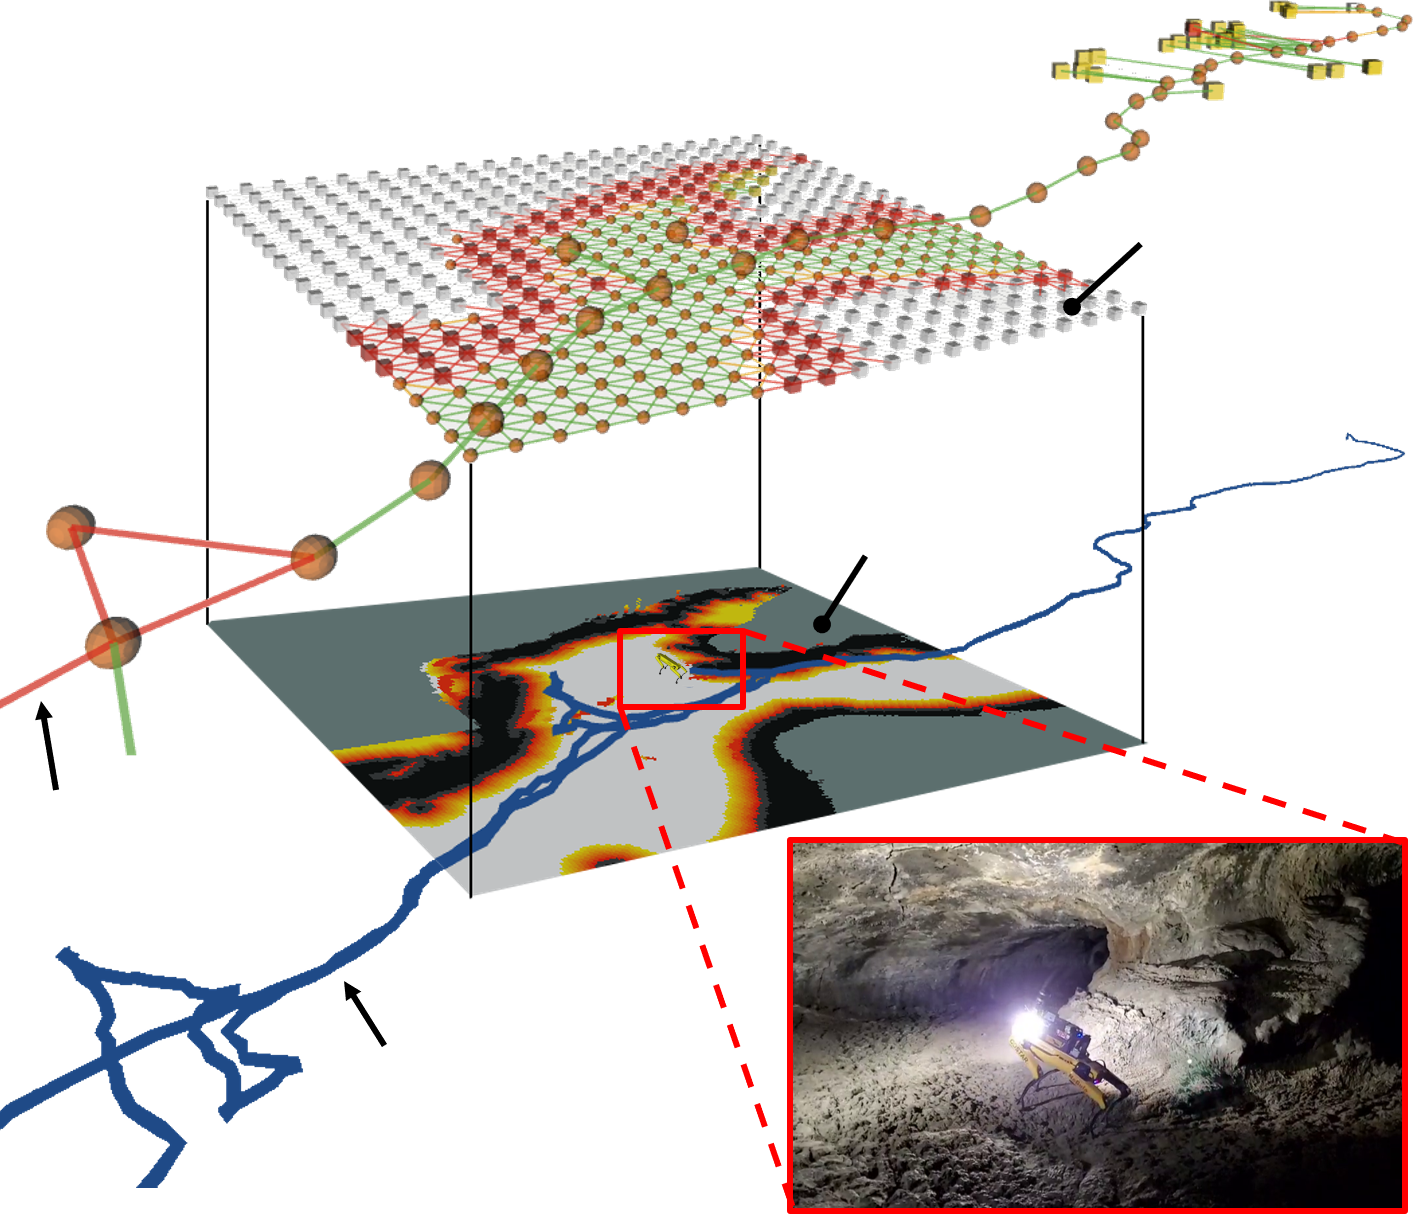
\includegraphics[width=1\columnwidth]{figures/hierarchy_labels_spot.png}};
	    \begin{scope}[x={(image.south east)},y={(image.north west)}]
	    	
	    	% Annotations 
	    	\node [font=\scriptsize,above left,align=right,black] at (0.93,0.79) {Local IRM}; %{Lattice IRM};
	    	\node [font=\scriptsize,above left,align=right,black] at (0.7,0.54) {Riskmap}; %{Graph IRM};
	    	\node [font=\scriptsize,above left,align=right,black] at (0.38,0.08) {Pose Graph};
	    	\node [font=\scriptsize,above left,align=right,black] at (0.17,0.29) {Global IRM};

	    \end{scope}
	\end{tikzpicture}	
  \caption{Hierarchical Information RoadMaps (IRMs) generated during Au-Spot's autonomous exploration of Martian-analog caves at Lava Beds National Monument, Tulelake, CA.} \label{fig:IRMs} 
\end{figure}



From a value learning perspective, a coverage planning problem in an unknown space can be considered an active learning problem over the robot's belief, where belief is defined as the probability distributions over all possible joint robot-world states.
%
The objective is to find the best action sequence that maximizes the accumulated reward over time.  The agent must accumulate data to incrementally build a model of its environment, and need to understand the effects of its actions on the quality and quantity of data it collects.

\phdone{Problem description--POMDP perspective}
Since the agent's future actions affect its belief of the world and robot state, this coverage problem is fundamentally a Partially Observable Markov Decision Process (POMDP) problem~\cite{pomdps_monahan1982}.
%A POMDP is a principled formalization of 
%a sequential decision making process under motion and sensing uncertainty.
The agent employs the underlying intrinsic model of the sequential action-observation process under uncertainty, so that it can %(asymptotically) converge to the optimal solution in a more 
expand its search structure over the space and learn the value in a more sample-efficient manner than model-free learning approaches.
In addition, its non-myopic reasoning provides better performance than one-step look-ahead frontier selection approaches.

\phdone{Gap in the state-of-the-art}
Belief value learning in POMDP setting suffers from the curse of dimensionality \cite{KLC98} and curse of history \cite{Pineau03}. Many powerful methods extend the spatial and temporal horizons of POMDPs with varying degrees of efficiency and accuracy, e.g., \cite{silver2010monte,somani2013despot,bonet1998learning,kim2019pomhdp}. In this paper, we focus on exploration problems with very long time horizons (> 1 hour), large spatial extents (> 1 km), and high dimensional belief states (including beliefs on the state of the environment), that exacerbates the curses of history and dimensionality when planning robot behaviors over the belief space.
%

\phdone{Contributions}
To address this problem, we introduce spatial and temporal approximations of the robot policy space to enable computational tractability while constructing a real-time online solver.
%search space.  This decomposition allows us to approximately solve the optimization problem in a computationally tractable manner.  
Spatially, we decompose the belief space into task-relevant partitions of the space,
%into a robot and task-relevant graph structure 
enriched with environment map estimates. %, which reduces our search space for good policies, 
The partitioning structure is called an Information Roadmap (IRM) (see Fig.~\ref{fig:IRMs}). Temporally, we decompose the problem into a long-range (global) IRM which spans the entirety of the known environment, and a robot-centered short-range (local) IRM. % with fixed size. 
We then propose a Receding Horizon Planning (RHP)-based solver to address online planning over this hierarchical POMDP structure.
% problem in a receding horizon fashion, 
% in real time.
\acomm{Consider bullet points. Link each gap to a contribution in this paragraph.}

\phdone{Outline}
The remainder of this paper is as follows: Following the related work discussion, Section~\ref{sec:formulation} formalizes the planning problem. In Section~\ref{sec:plgrim}, we propose a hierarchical belief learning and a solver for the proposed coverage planning problem. Experimental results in simulation and on a physical robot are presented in Section~\ref{sec:exp_results}.% validating our method, and Section~\ref{sec:conclusion} concludes this paper.


%%%%%%%%%%%%%%%%%%%%%%%%%%%%%%%%%%%%%%%%%%%%%%%%%%%%%%%%%%%%%%%%%%%%%%%%%%%%%%%%
\section{Related Work}\label{sec:related_work}
\phdone{Coverage--Frontier-based exploration}
Frontier-based exploration is a widely used approach for autonomous exploration (e.g., \cite{yamauchi1997frontier,tao2007motion,keidar2012robot,heng2015efficient,gonzalez2002navigation,grabowski2003autonomous}). By continuing exploration until exhausting all remaining frontiers, frontier-based approaches can guarantee \textit{completeness} of the coverage of reachable spaces.  These methods typically rely on myopic (e.g., one-step) look-ahead greedy policies, selecting the best frontier upfront. Hence they can be subject to local minima and provide suboptimal solutions in time.

\phdone{Coverage--(Model-free) RL-based approaches}
Model-free reinforcement learning (RL) has been applied to coverage and exploration problems (e.g., \cite{pathak_icm, rnd,burda2018study,ECR2018}). In this setting, the typical approach is to find a policy which maps sensor data to actions, with the objective of maximizing the reward. When it comes to long-range and large-scale, and (possibly safety-critical) missions on physical robots, collecting necessary data can be a significant challenge for this class of methods.

\phdone{Coverage--(Model-based RL) POMDP approaches}
POMDP-based approaches generate a non-myopic policy by considering long-horizon action sequences (e.g., \cite{kurniawati2011motion}, \cite{bai2015intention}), interactively learning the value function, and returning the best action sequence that maximizes the accumulated rewards. Different methods have reduced the complexity of the POMDP problem in coverage and exploration problems. \citet{indelman2015planning} and \citet{martinez2009bayesian} employed a direct policy search scheme with a Gaussian belief assumption. \citet{Lauri2016planning} extended this to non-Gaussian beliefs using the POMCP (Partially Observable Monte-Carlo Planning) solver. % algorithm that uses a Monte-Carlo Tree Search \cite{silver2010monte}.
%In this work, we aim at scaling the solution even further to enable solutions for hte missions fo interste that are longer and larger than mission 
However, when it comes to the large-scale coverage missions discussed in Section \ref{sec:intro}, the current approaches do not scale well due to the curse of history and dimensionality \cite{Pineau03}.

\phdone{Large scale--Hierarchical approaches}
Hierarchical planning structures \cite{kaelbling2011planning} aim to tackle larger problems by employing multiple solvers running at different resolutions.  
%
In the coverage and exploration context, \citet{umari2017autonomous} applies hierarchical planning to frontier-based exploration, while  \cite{dang2019explore} extends the lower level module to a more sophisticated frontier selection algorithm which considers the information gain along each path. \citet{Lauri2016planning} replace the lower level module with a POMDP-based planner, to improve local coverage performance with non-myopic planning. \citet{kim2019bi} propose a hierarchical online-offline solver for risk-aware navigation. \citet{vien2015hierarchical} propose a hierarchical POMCP framework which outperformed Bayesian model-based hierarchical RL approaches in some benchmarks.


\section{Problem Formulation}
\label{sec:formulation}

Autonomous exploration in unknown environments under motion and sensing uncertainty can be formulated as a Partially Observable Markov Decision Process (POMDP), which is one of the most general models for sequential decision making.
In this section, we present the POMDP formulation of coverage problems and address the intrinsic challenges.

\subsection{Preliminaries}
\phdone{POMDP Elements}
A POMDP is described as a tuple $\langle \mathbb{S}, \mathbb{A}, \mathbb{Z}, T, O, R \rangle$, where $\mathbb{S}$ is the set of joint robot-and-world states, $\mathbb{A}$ and $\mathbb{Z}$ are the set of robot actions and observations.
At every time step, the agent performs an action $a \in \mathbb{A}$ and receives an observation $z \in \mathbb{Z}$ resulting from the robot's perceptual interaction with the environment.
% we can drop a few more words from the sentences below..
The motion model $T(s, a, s') = P(s'\,|\,s, a)$ defines the probability of being at state $s'$ after taking an action $a$ at state $s$.
The observation model $O(s, a, z) = P(z\,|\,s, a)$ is the probability of receiving observation $z$ after taking action $a$ at state $s$.
The reward function $R(s, a)$ returns the expected utility for executing action $a$ at state $s$.
In addition, a belief state $b_t \in \mathbb{B}$ at time $t$ is introduced to denote a posterior distribution over states conditioned on the initial belief $b_0$ and past action-observation sequence, i.e., $b_{t} = P(s \,|\, b_0, a_{0:t-1}, z_{1:t})$.

\phdone{POMDP Objective function}
% The objective function of a generic POMDP can be described as follows.
The optimal policy of a POMDP for all time $t \in [0,\infty)$, $\pi_{0:\infty}^* \! : \mathbb{B} \to \mathbb{A}$, is defined as
\begin{align}
  % \pi^*(b) &= \arg\max_\pi \, \mathbb{E} \sum_{t=0}^{L} \gamma^t r(b_t, \pi(b_t)),
  \pi_{0:\infty}^*(b) &= \argmax_{\pi \in \Pi_{0:\infty}} \, \mathbb{E} \sum_{t=0}^{\infty} \gamma^t r(b_t, \pi(b_t)),
  % \pi_{0:\infty}^*(b_0) &= \argmax_{\pi \in \Pi_{0:\infty}} \, \mathbb{E} \sum_{t=0}^{\infty} \gamma^t r(b_t, \pi(b_t)),
  % \pi_{0:\infty}^*(\cdot) &= \argmax_{\pi \in \Pi_{0:\infty}} \, \mathbb{E} \sum_{t=0}^{\infty} \gamma^t r(b_t, \pi(b_t)),
  \label{eq:objective_function}
\end{align}
where $\gamma \in (0, 1]$ is a discount factor for the future rewards, $\Pi_{0:\infty}$ is the space of possible policies, and $r(b,a)=\int_s R(s,a)b(s)\mathrm{d}s$ denotes a belief reward which is the expected reward of taking action $a$ at belief $b$. \acomm{Ali says define $\pi$, but $\pi$ is just sampled from space of all policies$\Pi_{0:\infty}$?}


% \subsection{Unknown Environment Coverage Problem Formulation}
\subsection{Coverage Problem in Unknown Environments}

\phdone{Coverage Problem}
For coverage planning problems, we define the state $s$ as a tuple of robot $q$ and world states $W$, i.e., $s = (q, W)$.
We further decompose $W$ as states that can be explored or covered by the robot ($W_{cov}$), and states that are cannot be covered because they are occupied by obstacles ($W_{occ}$). % give examples? building, trees, rocks, etc?

A reward function for coverage can be defined as a function of information gain $I$ and action cost $C$ as
\begin{align}
  % R(s, a) = f(I(z(s, a), W_{cov}),\; C(q, a, W_{occ})),
  % R(s, a) = f(I(W_{cov}, z),\; C(W_{occ}, q, a)),
  R(s, a) = \mathrm{fn}(I(W_{cov}, z),\; C(W_{occ}, q, a)),
  \label{eq:coverage_reward}
\end{align}
% where $I(z, W_{cov})$ and $C(q, a, W_{occ})$ are functions of $W_{cov}$ and $W_{occ}$, respectively.
% where $I(W_{cov}, z)$ and $C(W_{occ}, q, a)$ are functions of $W_{cov}$ and $W_{occ}$, respectively.
where $I(W_{cov}, z) = H(W_{cov}) - H(W_{cov} \,|\, z)$ is the reduction in entropy $H$ of $W_{cov}$ after observation $z$.  %% practically, z would contain the lidar sensor readings with the current robot pose estimation, so no need for q as an input argument for I
$C(W_{occ}, q, a)$ is evaluated from actuation efforts and risks to take action $a$ at robot state $q$ on $W_{occ}$.
% More detailed definitions are presented in Section~\ref{sec:plgrim} [TODO: ref to subsection].

\phdone{Receding Horizon Planning}
In unknown space-coverage domains, the knowledge about $W_{cov}$ and $W_{occ}$ at run time is incomplete and often inaccurate, because we do not know which parts of the world we do not know.
% By plugging Eq.~(\ref{eq:coverage_reward}) into Eq.~(\ref{eq:objective_function}), we can formulate the coverage planning problem with an infinite planning horizon in a POMDP setting.
% Then we can identify several fundamental challenges to solve this problem.
%
Thus, it is fundamentally infeasible to solve an unknown environment coverage problem when formulated for an infinite horizon, as in Eq.~(\ref{eq:objective_function}).

\phdone{RHP Objective Function}
Instead, a Receding Horizon Planning (RHP) scheme has been widely adopted in most of the state-of-the-art formulations \cite{bircher2016receding}.
In this POMDP-RHP formulation, the infinite-horizon optimal policy from Eq.~(\ref{eq:objective_function}) is altered to execute for a finite horizon $T$. This execution from time $t$ to $t+T$ is known as a planning episode.
\begin{align}
  \pi_{t:t+T}^*(b) &= \argmax_{\pi \in \Pi_{t:t+T}} \, \mathbb{E} \sum_{t'=t}^{t+T} \gamma^{t'-t} r(b_{t'}, \pi(b_{t'}))
  \label{eq:receding_objective_function}
\end{align}
Given the policy for previous planning episode, only a part of the optimal policy, $\pi^*_{t:t+\Delta t}$ for $\Delta t \in (0, T]$, will be executed at run time. A new planning episode will start at time $t+\Delta t$ with the updated $W_{cov}$, $W_{occ}$ and reward $R(s,a)$.
% [TODO: Additional notes on RHP]

% [\sout{NOTE: $\Delta t$ and $T$ can also be variables.} Assume them to be constant here.]

% NOTE: receding horizon planning for info gain rewards; no reference trajectory, reward function is past action-observation sequence dependent, possibly multiple optimal solutions if without previous path info

% [NOTE: The range for $W_{cov}$ update is often smaller than that for $W_{occ}$ update. For example, from the same sensor readings (like lidar), $W_{occ}$ is updated up to 20m from the current robot position, while $W_{cov}$ is updated up to 4m based on the conservative coverage sensor model.]

% [NOTE: coverage problem cannot be formulated as a Markov Decision Process (MDP) as our state space is not fully known, especially the world state. The reward function, depending on the state, also depends on the history of action-observation sequences. For example, once the robot had explored a local area and gathered the information gain, then it will get additional information gain even though it revisits that area again and again.]

% Due to the nature of unknown space exploration with limited field of view,
% receding horizon planning with optimism in the face of uncertainty or KWIK (know what it knows) [cite]
% revised objective function for coverage with a finite receding horizon


\subsection{Challenges} \label{ssec:challenges}
% Solving the POMDP-RHP coverage problem in Eq.~(\ref{eq:receding_objective_function}) necessitates balancing conflicting planner requirements: long time horizons and high resolution action spaces, as well as consistency and resiliency between successive plans.

% Environment:
% - Unknown 
%     - Reliance on noise-susceptible belief 
%     - Receding-horizon introduces consistency vs. resiliency trade-off:
%         - Path consistency between episodes
%         - Path resilience to inaccurate information
    
% - Large
%     - Memory efficient world representation (computationally constrained)

% - Difficult Terrain
%     - precision --> high resolution action sequence (computationally constrained)
%     - myopic could be risky? not really

% Objective:
% - Coverage
%     - efficiency --> long horizon action sequence (computationally constrained)
 
%  The agent must understand how its actions affect the coverage belief state. 
   
We detail the challenges associated with solving the coverage planning problem in an unknown, large ($> 1~km$), and rugged-terrain environment over long-time scales ($> 1~hr$) using a POMDP-RHP formulation. We categorize these challenges as computational---time complexity, space complexity---or trajectory-concatenation/blah specific.

\ph{Time Complexity}
POMDP planning suffers from two computationally-constrained phenomena: \textit{curse of dimensionality} and \textit{curse of history}. The former difficulty is sourced in the fact that the state space grows exponentially with the number of state variables, and the the time complexity of a belief update is quadratic in the size of the state space: $\mathcal{O}(|\mathbb{S}|^2)$. The latter difficulty refers to the fact that the number of action-observation histories scales with the product of the action- and observation-space sizes, and the time complexity of evaluating all action-observation histories is exponential in planning depth $D$: $\mathcal{O}((|\mathbb{A}||O|)^D)$. Together, both \textit{curses} result in a POMDP planning time-complexity of $\mathcal{O}((|\mathbb{A}||O|)^D|\mathbb{S}|^2)$. As a concrete example - in order to plan a coverage trajectory spanning $1~hr$ through a $1~km$ environment with precise motions that negotiate rugged terrain ($1~m$ motions into the eight cardinal and inter-cardinal directions), the time complexity (assuming no belief update) is $\mathcal{O}((|8||1000*1000|)^{1000})$ (probably wrong). In practice, given limited onboard computational resources and online time constraints, we can't solve this problem, since planning time available may be short, especially since we're entering unknown area and terrain is difficult so we are very vulnerable to sensor and movement uncertainty blah blah blah, real-time system constraint.

\ph{Space Complexity}
The memory (or space complexity?) required to store the world state, used by the planning algorithm, is dictated by the environment size, map resolution, number of world state variables ($W_{occ}, W_{cov}$), and the fidelity of the variables' values (e.g. Boolean vs. floating-point): $\mathcal{O}(|n|^2)$ where $n$ is the map size. As a concrete example, assuming use of a grid structure, the memory required to represent a $1~km$ environment at a $0.1~m$ resolution, where each cell stores occupancy and coverage probabilities (floating-point), is: . 






$\mathcal{O}(|n|^2)$, and assuming we have a double-type value

 A memory-efficient world representation that stores high-fidelity information about the entire known environment, which can be queried when solv-ing for the long-horizon coverage policy.


POMDP complexity -> relationship between factors (horizon, branching factors-action space, observation space-belief space resolution)
O((|action| * |observation|)^depth)

**Constraints (computational-time complexity, memory-space complexity) --> CLARIFICATION WITH OTHER PEOPLE (Kyon?)
--> Curse of dimensionality/history

Our case:
* Time complexity
Space > 1km
action (motion) resolution ~ 1m  *with the help of local motion planner
action set: 8-neighbor (orientation?)
observation: Gaussian-type? 0/1 FOV-sensor model? --> Combination of obstacle cells in FOV: O(2^(5x5)) for FOV 5m --> (Relevant to Memory)
Depth ~ 1000 steps
--> O((8*1000)^1000) --> blows up!


% A* algorithm
% 100x100 cells --> how much of cells should be memorized at a time (space complexity)

* Memory --> per O(1) each operation % (not very tightly related to algorithm's space complexity)
Representation of W_occ, W_cov

General:
Occupancy % (traversability) (--> edge connection)
Coverage % (IG) (--> Frontier)

Our case:
Real-time system constraint?

0.1m resolution costmap
1km for this resolution
(1e5)^2 in 2D representation
1 cell in double-type --> 4byte? --> ?GB x2 (occ, cov) --> blows up!




We detail the challenges associated with solving the coverage planning problem in an unknown, large (> 1 km), and rugged-terrain environment over long-time scales (> 1 hr) using a POMDP-RHP formulation. We categorize these challenges as...

Hierarchical (1), Roadmap (2)
- Curse of Dimensionality: in partially observable environment, agent must reason in space of beliefs (probability distributions over states). If agent naively discretizes belief space, the number of discrete beliefs then grows exponentially with the number of states.
    - Large Environment
    - Rugged-terrain

POMDP Solver (3)
- Curse of History: number of action-observation histories grows exponentially with the planning horizon.
    - Globally: Large environment, Long time scales
    - Locally: High resolution state space

Hierarchical (1), Roadmap (2)
- Memory Efficient Representation
    - Large Environment
    - Rugged-terrain
    - Long time scales

safety-critical RH implementation (4)
- Receding Horizon: incomplete information / how to deal with updating belief
    - Consistency between episodes --> path concatenation assuming belief is accurate
    - Resilience to noise
    
    
    
    
% Smart discretization of belief space

% - long time horizons (> 1 hour)
% - large spatial extents (> 1 km)
% - high dimensional belief states

% Objective: Coverage 
% - Efficiency --> long horizon action sequence

% Environment attribute: Unknown 
% What's difference between belief and RH in terms of motivation?
% - Incomplete information --> Receding Horizon Implementation 
%     - Consistency between episodes --> path concatenation assuming belief is accurate
%     - But what if belief is not accurate? This leads to resilience
% - Belief --> noise susceptible --> Bad information
%     - Resilience to noise
    
% Environment attribute: Large 
% - Memory efficient representation
% - Long horizon

% Environment attribute: Rugged-Terrain 
% - High resolution action sequence


Efficient exploration of a large-scale environment with complex terrain requires reasoning over long temporal horizons while maintaining the ability to locally plan precise motions that can negotiate complex terrains. These two requirements---optimal action sequences spanning the known environment and high resolution action spaces---are incompatible given a robot's limited onboard computational resources during real-time planning. Therefore, the solver and action space must be designed with this resource-constraint (conflict) in mind. Furthermore, limited computational resources also necessitate a memory-efficient world representation that stores high-fidelity information about the entire known environment, which can be queried when solving for the long-horizon coverage policy. 
 
\ph{Plan Consistency vs. Resiliency}
Action sequences generated during consecutive planning iterations must respect the dynamic constraints of the robot (consistency), while simultaneously adapting to unexpected hazards in the environment (resiliency). As was the case with long horizon and high resolution planning objectives, plan consistency and resiliency are often in opposition. Unexpected changes in the local world representation, due to sensor data delays or map prediction errors, may require aggressive maneuvers to avoid a collision. However, if the maneuver violates a robot's motion constraints (e.g., minimum turning radius), then the robot may destabilize and become inoperable. Thus, finding a balance between plan consistency and resiliency, particularly for safety-critical systems operating in natural disaster areas, is vital so that a coverage mission does not end prematurely due to physical robot failure. 



%%%%%%%%%%%%%%%%%%%%%%%%%%%%%%%%%%%%%%%%%%%%%%%%%%%%%%%%%%%%%%%%%%%%%%%%%%%%%%%%
\section{PLGRIM: Hierarchical Coverage Planning on Information Roadmaps}
\label{sec:plgrim}

\phdone{Framework Overview}
In this section, we present a novel and field-hardened autonomy framework, \textit{PLGRIM (Probabilistic Local and Global Reasoning on Information roadMaps)}, for exploration of large-scale unknown environments.
% Our key ideas to tackle the challenges described in Section~\ref{ssec:challenges} are as follows:

We now present our key ideas to tackle the challenges described in Section~\ref{ssec:challenges}:
% To handle the \textit{Planner Horizon vs. Resolution} tradeoff:


\vspace{-4pt}
\begin{enumerate}[label={\arabic*)}]
  \itemsep0em 
  \setlength{\itemsep}{0pt}
  \setlength{\parskip}{0pt}
  \item \label{en:idea1} We propose a hierarchical belief manager/planner structure to scale up to spatially large problems.
  \item \label{en:idea2} At each hierarchical level, we maintain and represent the belief about the world in a compact and versatile form, called Information RoadMap  or IRM.
  \item \label{en:idea3} We employ efficient POMDP solvers adequate for each hierarchical level to reason over a longer temporal horizon within the given replanning time.
  \item \label{en:idea4} We extend the Receding Horizon Planning (RHP) scheme to provide consistent and resilient coverage planning for safety-critical systems.
\end{enumerate}
\vspace{-4pt}

% \noindent Finally, we extend the Receding Horizon Planning (RHP) scheme to provide consistent and resilient coverage planning for safety-critical systems (\textit{Plan Consistency vs. Resiliency} tradeoff).

% \begin{enumerate}[label={\arabic*)}]
%   \item We extend the Receding Horizon Planning (RHP) scheme to provide consistent and resilient coverage planning for safety-critical systems (Challenge~\ref{en:issue3a} and \ref{en:issue3b}).
% \end{enumerate}
Proposals~\ref{en:idea1}~through~\ref{en:idea3}~address the \textit{Planner Horizon vs. Resolution} challenge, while proposal~\ref{en:idea4}~addresses the \textit{Plan Consistency vs. Resiliency} challenge. In the following subsections, we provide the technical details about the proposed framework.

% (subsections)
% 4.1. Hierarchical Belief Space Representation -- Compact world representation (IRM): 1.b
% 4.2. Hierarchical Coverage Policy Formulation -- Hierarchical world representation and planning structure: 2.a, (1.b)
% 4.3. Efficient/Real-time (Hierarchical) POMDP solvers --  Efficient POMDP solver (QMDP, POMCP): 2.b
% 4.4. Consistent and resilient planning (RHP formulation + adaptation): 3.a-b


\subsection{Hierarchical POMDP Policy Formulation}
\label{ssec:hierarchical_policy}

\begin{figure}[t!]
\centering
    \begin{tikzpicture}
    \node[anchor=south west,inner sep=0] (image) at (0,0) {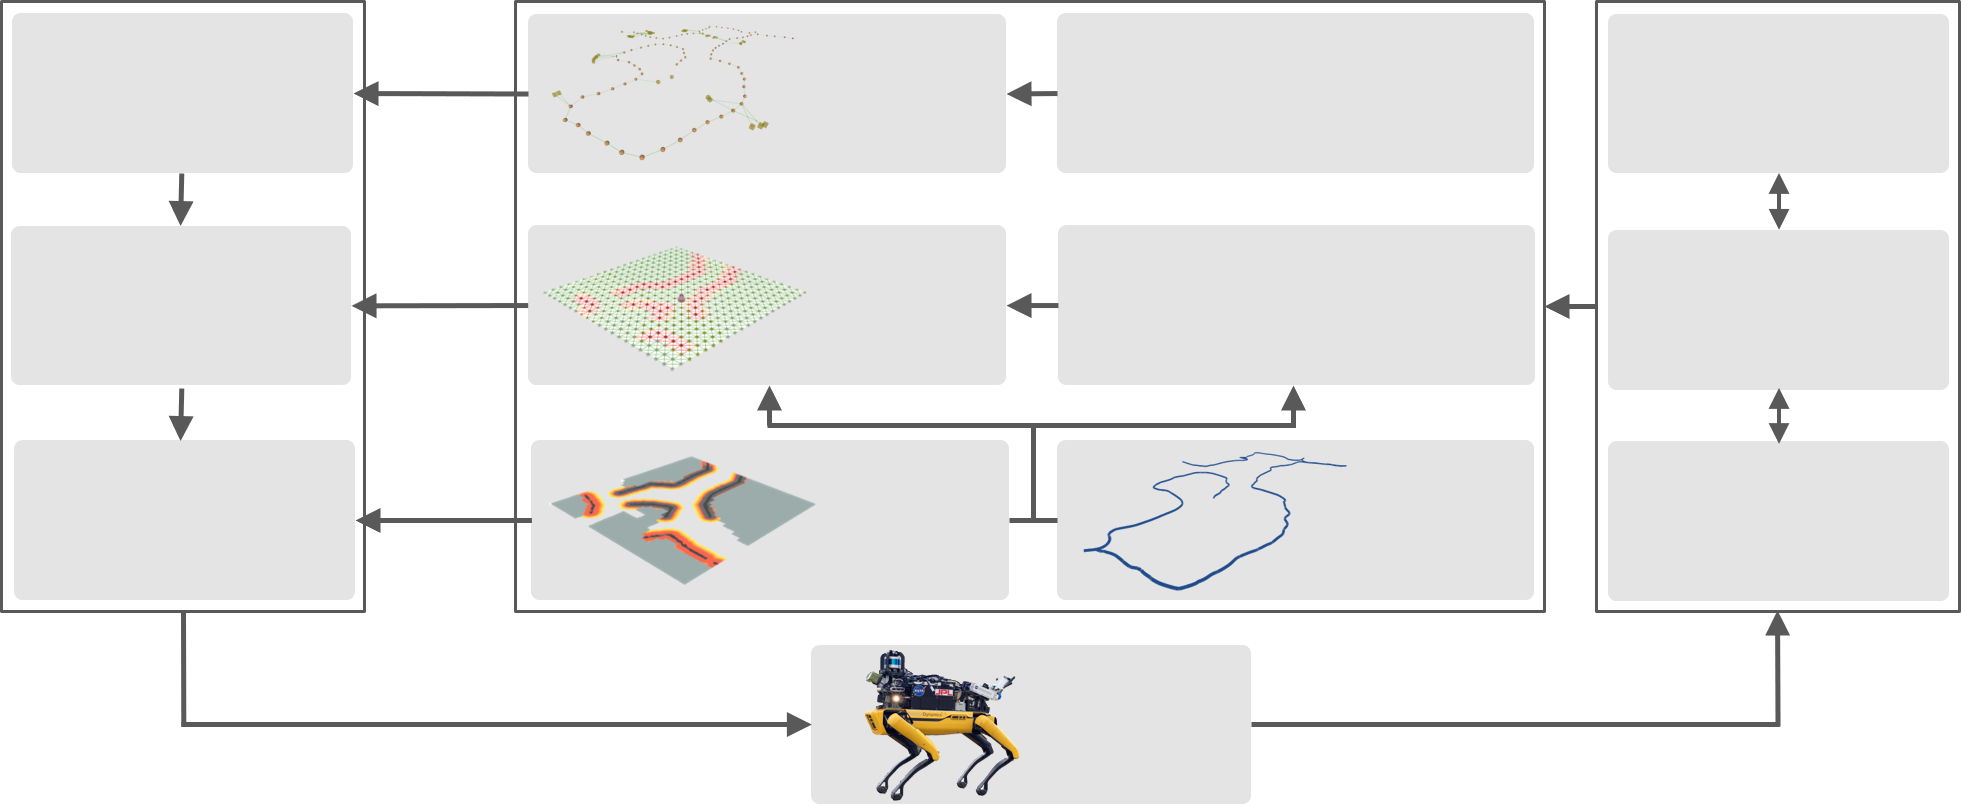
\includegraphics[width=1\columnwidth]{figures/diagram_v16.png}};
	    \begin{scope}[x={(image.south east)},y={(image.north west)}]
	    	
	    	% Annotations 
	    	\node [font=\tiny,above left,align=right,black] at (0.265,0.61) {Local};
	    	\node [font=\tiny,above left,align=right,black] at (0.264,0.53) {IRM};
	    	\node [font=\tiny,above left,align=right,black] at (0.275,0.87) {Global}; 
	    	\node [font=\tiny,above left,align=right,black] at (0.264,0.79) {IRM}; 
	    	\node [font=\tiny,above left,align=right,black] at (0.265,0.255) {Risk\\Map}; 
	    	
	    	\node [font=\scriptsize,above left,align=right,black] at (0.99,0.54) {Odometry}; 
	    	\node [font=\scriptsize,above left,align=right,black] at (1,0.81) {3D Mapping}; 
	    	\node [font=\scriptsize,above left,align=right,black] at (1,0.28) {Traversability}; 	
	    	
	    	\node [font=\scriptsize,above left,align=right,black] at (0.76,0.59) {Path Traversal}; 
	    	\node [font=\scriptsize,above left,align=right,black] at (0.73,0.52) {Checker}; 
	    	\node [font=\scriptsize,above left,align=right,black] at (0.72,0.86) {Frontier}; 
	    	\node [font=\scriptsize,above left,align=right,black] at (0.73,0.77) {Manager}; 
	    	\node [font=\scriptsize,above left,align=right,black] at (0.77,0.33) {Pose}; 
	    	\node [font=\scriptsize,above left,align=right,black] at (0.78,0.25) {Graph}; 
	    	
	    	\node [font=\tiny,above left,align=right,black] at (0.52,0.85) {Global IRM}; 
	    	\node [font=\tiny,above left,align=right,black] at (0.51,0.78) {Manager}; 
	    	\node [font=\tiny,above left,align=right,black] at (0.52,0.59) {Local IRM}; 
	    	\node [font=\tiny,above left,align=right,black] at (0.51,0.51) {Manager}; 
	    	\node [font=\scriptsize,above left,align=right,black] at (0.508,0.33) {Risk}; 
	    	\node [font=\scriptsize,above left,align=right,black] at (0.51,0.25) {Map}; 
	    	
	    	\node [font=\scriptsize,above left,align=right,black] at (0.38,0.08) {Velocity Commands};
	    	\node [font=\scriptsize,above left,align=right,black] at (0.85,0.08) {Sensor Data};
	    	\node [font=\scriptsize,above left,align=right,black] at (0.63,0.05) {Robot};
	    	
	    	\node [font=\tiny,above left,align=right,black] at (0.193,0.85) {Global Coverage};
	    	\node [font=\tiny,above left,align=right,black] at (0.15,0.8) {Planner};
	    	\node [font=\tiny,above left,align=right,black] at (0.188,0.58) {Local Coverage};
	    	\node [font=\tiny,above left,align=right,black] at (0.15,0.53) {Planner};
	    	\node [font=\tiny,above left,align=right,black] at (0.18,0.32) {Kinodynamic};
	    	\node [font=\tiny,above left,align=right,black] at (0.15,0.27) {Planner};
	    	
	    	\node [font=\scriptsize,above left,align=right,black] at (0.15,0.97) {Planner};
	    	\node [font=\scriptsize,above left,align=right,black] at (0.67,0.96) {Belief Value Manger};
	    	\node [font=\scriptsize,above left,align=right,black] at (0.98,0.97) {Inference};

	    \end{scope}
	\end{tikzpicture}	
  \caption{Planner framework enabling Hierarchical Information RoadMaps (IRMs) for large-scale exploration in unknown environments.} \label{fig:framework} 
\end{figure}




\phdone{Formulation}
First, we formulate the hierarchical coverage planning in a POMDP setting.
%
% Let us decompose a belief state $b$ into local and global belief states, $b^\ell = (q, W^\ell)$ and $b^g = (q, W^g)$, respectively,
% Let us decompose a belief state $b$ into local and global belief states, $b^\ell = P((q, W^\ell))$ and $b^g = P((q, W^g))$, respectively.
Let us decompose a belief state $b$ into local and global belief states, $b^\ell = P(q, W^\ell)$ and $b^g = P(q, W^g)$, respectively.
$W^\ell$ is a local, rolling-window world representation with high-fidelity information, while $W^g$ is a global, unbounded world representation with approximate information (see Fig.~\ref{fig:IRMs}).

With $\pi^\ell$ and $\pi^g$ denoting the local and global policies, respectively, we approximate the original RHP optimization problem in Eq.~(\ref{eq:receding_objective_function}) as cascaded hierarchical optimization problems as follows:
\begin{align}
  &\pi_{t:t+T}(b)
  = \argmax_{\pi \in \Pi_{t:t+T}} \, \mathbb{E} \sum_{t'=t}^{t+T} \gamma^{t'-t} r(b_{t'}, \pi(b_{t'}))
  % = \argmax_{\pi^\ell \in \Pi^\ell_{t:t+T}} \, \mathbb{E} \sum_{t'=t}^{t+T} \gamma^{t'-t} r(b_{t'}, \pi^\ell(b^\ell_{t'}; \theta^\ell))
  \nonumber \\
  & \approx \argmax_{\pi^\ell \in \Pi^\ell_{t:t+T}} \, \mathbb{E} \sum_{t'=t}^{t+T} \gamma^{t'-t} r^\ell(b^\ell_{t'}, \pi^\ell(b^\ell_{t'}; \pi_{t:t+T}^g(b^g_t))),
  \label{eq:llp_optimization}
  \\
  &\text{where }
%   \pi_{t:t+T}^g(b^g) = \argmax_{\pi^g \in \Pi^g_{t:t+T}} \, \mathbb{E} \sum_{t'=t}^{t+T} \gamma^{t'-t} r^g(b^g_{t'}, \pi^g(b^g_{t'}))
  \pi_{t:t+T}^g(b^g) = \argmax_{\pi^g \in \Pi^g_{t:t+T}} \, \mathbb{E} \sum_{t'=t}^{t+T} \gamma^{t'-t} r^g(b^g_{t'}, \pi^g(b^g_{t'})).
  \label{eq:glp_optimization}
%   \label{eq:optimal_policy_unified}
\end{align}
\normalsize
% $\tilde{r}(b^g, \pi^g(b^g))$ is an approximate belief reward function for the global belief space.
$r^\ell(b^\ell, \pi^\ell(b^\ell))$ and $r^g(b^g, \pi^g(b^g))$ are approximate belief reward functions for the local and global belief spaces, respectively.
%
Note that the codomain of the global policy $\pi^g(b^g)$ is a parameter space $\Theta^\ell$ of the local policy $\pi^\ell(b^\ell; \theta^\ell)$, $\theta^\ell \!\! \in \! \Theta^\ell\!$.\,

\phdone{Section Structure}
According to this formulation, we maintain the hierarchical belief representations (Section~\ref{ssec:belief-managers}) and solve for hierarchical POMDP policies (Section~\ref{ssec:belief-planners}).
For local planning consistency and resiliency, we extend Eq.~(\ref{eq:llp_optimization}) to a joint optimization problem given the previous planning episode policy (Section~\ref{ssec:resilient_rhp}).
% See Algorithm~\ref{alg:PLGRIM} for algorithmic description of the overall framework.

% Section 4.2: how to form local and global belief space 
% Section 4.3: how to solve optimization at each level
% Section 4.4: how to enhance the resiliency in the lower level



% \subsection{Hierarchical Belief Managers} \label{ssec:belief-managers}
\subsection{Hierarchical Belief Representation} \label{ssec:belief-managers}
\begin{algorithm}[t!]
% {\fontsize{9.2pt}{10.6pt}\selectfont
{\fontsize{8.5pt}{9.8pt}\selectfont
\caption{PLGRIM: Hierarchical IRM Construction}
% \caption{PLGRIM: Information Roadmap Construction}
\label{alg:IRMs}
\begin{algorithmic}
  \STATE \textbf{input:} Riskmap, Pose Graph %, (estimated) robot pose %, Odometry

  \vspace{3pt}
  % \STATE \textbf{\# Local IRM}
  \STATE \textbf{\textit{\# Local IRM}}
  \STATE Local IRM $G^\ell = (N^\ell, E^\ell) \gets (\emptyset, \emptyset)$
  \STATE Add uniformly sampled nodes $\{\hat{w}^\ell_i\}_i$ around the robot to $N^\ell$
  \FOR {each $\hat{w}^\ell_i \in N^\ell$}
    % \STATE Compute occupancy probability $P(\hat{w}^\ell_{i,occ})$ from Riskmap
    % \STATE Compute coverage probability $P(\hat{w}^\ell_{i,cov})$ from Riskmap and Pose Graph by ray tracing
    \STATE Compute occupancy probability $P(\hat{w}^\ell_{i,occ})$ and coverage probability $P(\hat{w}^\ell_{i,cov})$ from Riskmap and Pose Graph for $\hat{w}^\ell_i$
    \STATE Add $P(\hat{w}^\ell_{i,occ})$ and $P(\hat{w}^\ell_{i,cov})$ to the properties of $\hat{w}^\ell_i$
  \ENDFOR
  \STATE Add edges for 8-connected neighbors, $\{e_{ij}\}^\ell_{i,j}$, to $E^\ell$
  \FOR {each $e^\ell_{ij} \in E^\ell$}
    \STATE Compute traversal risk $\rho_{ij}$ and distance $d_{ij}$ for $e^\ell_{ij}$
    \STATE Add $\rho_{ij}$ and $d_{ij}$ to the properties of $e^\ell_{ij}$
  \ENDFOR

  \vspace{3pt}
  % \STATE \textbf{\# Global IRM}
  \STATE \textbf{\textit{\# Global IRM}}
  \IF {not initialized}
    \STATE Global IRM $G^g = (N^g_b \cup N^g_f, E^g) \gets (\emptyset, \emptyset)$
    % \STATE initialized $\gets$ True
  \ENDIF
  
  \STATE Get the current robot pose $q$ from Pose Graph
  \IF {$q$ is farther from any breadcrumb node $\forall \hat{w}^g_i \in N^g_b$ than $\bar{d}_b$}
%   \IF {$d(q, \hat{w}^g) > \bar{d}_b$ for $\forall \hat{w}^g \in N^g_b$}  % TODO: $d(\cdot, \cdot)$: distance function
    \STATE Add a new breadcrumb node $\hat{w}^g = q$ to $N^g_b$
  \ENDIF


%   \STATE Get frontier nodes to add, $\hat{N}^g_{f^+}$, and frontier nodes to prune, $\hat{N}^g_{f^-}$, from FrontierManager given Riskmap and Pose Graph
  \STATE Run Frontier Manager to add new frontiers $\{\hat{w}^g_{f^+}\}$ with coverage probabilities $\{P(\hat{w}^g_{f^+,cov})\}$, and prune invalidated frontiers, $\hat{w}^g_{f^-}$, based on the current Riskmap and Pose Graph
  \STATE \hspace{4.5cm} $\triangleright$ \cite{keidar2012robot}

  \FOR {each node $\hat{w}^g_i \in \mathcal{N}_{G^g}(q)$}
%   \STATE $\triangleright \mathcal{N}_{G^g}(q)$: Nearby nodes of q in $G^g$
    % \STATE Compute the traversal distance $d_{ij}$ and risk $\rho_{ij}$ to its nearby nodes $\forall \hat{w}^g_j \in \mathcal{N}_{G^g}(q)$
    \FOR {each nearby node $\hat{w}^g_j \in \mathcal{N}_{G^g}(\hat{w}^g_i)$}
      \STATE Compute the traversal distance $d_{ij}$ and risk $\rho_{ij}$
      \IF {$d_{ij} < \bar{d_e}$ and $\rho_{ij} < \bar{\rho_e}$}
        \STATE Add an edge $e^g_{ij}$ to $E^g$ with properties $d_{ij}$ and $\rho_{ij}$
      \ELSE
        \STATE Remove the edge $e^g_{ij}$ from $E^g$
      \ENDIF
    \ENDFOR
  \ENDFOR



  \vspace{3pt}
  \RETURN $G^\ell$ and $G^g$

\end{algorithmic}
} %fontsize environment
\end{algorithm}



\phdone{Data structure}
For compact and versatile representation of the world, we choose a generic graph structure, $G = (N, E)$ with nodes $N$ and edges $E$, as the data structure to represent the belief about the world state.
% [NOTE: Avoid using $V$ to denote the set of nodes as $V$ is reserved for the value function.]
We refer to this representation as an Information RoadMap (IRM).
We construct and maintain IRMs at two hierarchical levels, namely, Local IRM and Global IRM.
In this subsection, we provide a formal description how these IRMs encode the information about $W_{occ}$ and $W_{cov}$ at each level.


\phdone{Formulation}
We denote the ground-truth world state by $W^*$. When exploring unknown environments, at any given time, the robot's knowledge is limited to a subset of the  world $\hat{W}\!\!\subseteq\! W^*$ that has been explored and observed by the robot so far.
% In the unknown environment exploration domain, the ground-truth world state $W^*$ is not accessible at run time.
% Instead, we only have access to a subset of the world, $\hat{W} \subseteq W^*$, that has been explored and observed by the robot so far.
$\hat{W}$ has two distinct attributes, $\hat{W}_{occ}$ and $\hat{W}_{cov}$, that represent the occupancy and coverage states, respectively.
%
For $\hat{W} = \{\hat{w}_i\}_i$ where $\hat{w}_i$ is an individual spatial point in $\hat{W}$, we define $P(\hat{W}_{occ}) = \Pi_i P(\hat{w}_{i,occ})$ and $P(\hat{W}_{cov}) = \Pi_i P(\hat{w}_{i,cov})$ under the assumption of independence between the spatial points.
Additionally, let us denote the local patch of $\hat{W}$ around the robot by $\hat{W}^\ell$.
%
% (optional) the following holds:
% $W^* = W^*_{occ} \cup W^*_{\neg occ} = W^*_{cov} \cup W^*_{\neg cov}$.
%
% We assume/conjecture the independence between $W_{occ}$ and $W_{cov}$, i.e.,
% \begin{align}
%   P(W) &= P(W_{occ}, W_{cov}) \approx P(W_{occ}) P(W_{cov})
%   \label{eq:W_independence}
% \end{align}


\phdone{Information Sources}
Information to construct IRMs is sourced from other subsystems (see Fig.~\ref{fig:framework}).
A \textit{Riskmap} is a local rolling-window map that provides the risk assessment from the range sensor readings, %for a robot to be placed at each point of the map, 
which effectively encodes $P(\hat{W}^\ell_{occ})$.
% It provides not only the estimated risk but also the confidence of the estimation for each point.
% A \textit{Pose Graph} is a simple graph structure from SLAM (Simultaneous Localization and Mapping) module that provides the robot's past trajectory in global frame, 
A \textit{Pose Graph} %, provided by the SLAM (Simultaneous Localization and Mapping) module, 
provides the robot's past trajectory in the global coordinate frame, where $P(\hat{W}_{cov})$ can be inferred from.


\phdone{Local IRM}
% An algorithmic description about Local and Global IRM construction is presented in Algorithm~\ref{alg:IRMs}.
%
A Local IRM $G^\ell$ is rather straightforward to construct given a Riskmap and a Pose Graph.
Once we have uniformly down-sampled nodes at $\{\hat{w}^\ell_i\}_i \subset \hat{W}^\ell$,
we compute $P(\hat{w}^\ell_{i,occ})$ and $P(\hat{w}^\ell_{i,cov})$ from the Riskmap and Pose Graph for each node and encode them as node properties.
For each edge to a neighbor node we compute a traversal risk and distance that effectively encodes $\hat{W}^\ell_{occ}$ information between the two nodes.
Hence, a Local IRM contains relatively high-fidelity information with a high resolution, but locally.



\phdone{Global IRM}
Construction of a Global IRM $G^g$ needs more care, so that it can scale up to large $\hat{W}$, which may span up to several kilometers in this work.
Thus, instead of a densely sampled graph, we use a sparse graph structure for a Global IRM.
% A Global IRM is of a sparse graph structure, so that it can scale up to large $\hat{W}$, which may span up to several kilometers in this work.
%
It has two subsets of nodes, $N^g_b$ and $N^g_f$, so-called \textit{breadcrumb} and \textit{frontier} nodes, respectively, where $N^g_b \cap N^g_f = \emptyset$ and $N^g_b \cup N^g_f = N^g \! \subset \! \hat{W}$.
%
The breadcrumb nodes capture the \textit{covered free} space of $\hat{W}$, i.e., $N^g_b \subset \{\hat{w}_i | P(\hat{w}_{i,\neg occ} \wedge \hat{w}_{i,cov}) > \bar{\psi}_b\}$, while
the frontier nodes capture the \textit{uncovered free} space, i.e., $N^g_f \subset \{\hat{w}_i | P(\hat{w}_{i,\neg occ} \wedge \hat{w}_{i,\neg cov}) > \bar{\psi}_f\}$,
where $\bar{\psi}_b$ and $\bar{\psi}_f$ are some thresholds.
%
An additional condition for a candidate node $\hat{w}_i$ to be actually a breadcrumb or frontier node is that there should be a traversable path to nearby existing nodes in $G^g$, i.e., $\exists \hat{w}^g_j \in \mathcal{N}_{G^g}(\hat{w}_i)$ such that the traversal risk $\rho_{ij} \in [0, 1] < \bar{\psi}_e$ for $\hat{w}_i$ and $\hat{w}^g_j$, where $\mathcal{N}_{G^g}(\cdot)$ is a set of nearby nodes in $G^g$ and $\bar{\psi}_e$ is some threshold.
%
% In summary, we do not explicitly encode highly likely occupied, untraversable, or uncertain subspaces of $\hat{W}$ in a Global IRM for compact representation.
In short, a Global IRM captures the free-space connectivity with a notion of coverage, and does not explicitly encode highly likely occupied, untraversable, or uncertain subspaces of $\hat{W}$ for compact representation of the large-scale world.
%
For a detailed description of Global IRM construction process, see Algorithm~\ref{alg:IRMs}.




\subsection{Hierarchical Coverage Planning} \label{ssec:belief-planners}

Given Local and Global IRMs as the hierarchical belief representation, we solve the cascaded hierarchical POMDP problems, Eq.~(\ref{eq:llp_optimization}) and Eq.~(\ref{eq:glp_optimization}), for coverage in an unknown environment.



\phdone{General POMDP Solver Formulation}
We introduce some useful notations to describe the POMDP solvers.
% As can be seen in Eq.~(\ref{eq:objective_function}), the objective of 
The objective function of Eq.~(\ref{eq:objective_function}) in general is called a value function $V(b; \pi) = \mathbb{E} [\sum_t \gamma^t r(b_t, \pi(b_t))]$.
% Value function:
% % $V(b; \pi_{t:t+T0}) = \mathbb{E} [\sum_{t'=t}^{t+T} \gamma^{t'} r(b_{t'}, \pi_{t:t+T}(b_{t'}))]$
% $V(b; \pi) = \mathbb{E} [\sum_t \gamma^t r(b_t, \pi(b_t))]$
%
From a recursive form of the value function, we can define a Q-value function for a belief-action pair as follows:
\begin{align}
  Q(b, a; \pi) = r(b, a) + \sum_{b' \in \mathbb{B}} \gamma \mathcal{T}(b, a, b') V(b'; \pi),
  \label{eq:q_function}
\end{align}
where $\mathcal{T}(b, a, b') = \sum_{z \in \mathbb{Z}} P(b' | b, a, z) P(z | b, a)$ denotes the transition probability from $b$ to $b'$ by action $a$.
%
A POMDP solver tries to learn $Q(b, a)$ and $V(b) = \max_{a \in \mathbb{A}} Q(b, a)$, and returns the policy $\pi$ that specifies the best action for a given belief $b$, i.e., $\pi(b) = \argmax_{a \in \mathbb{A}} Q(b, a)$.


\phdone{Reward Function--Information Gain}
The reward function in Eq.~(\ref{eq:coverage_reward}) is concretely defined for our belief representation as follows.
A Local IRM $G^\ell = (N^\ell, E^\ell)$ contains $P(\hat{w}^\ell_{i,cov})$ value for each node $\hat{w}^\ell_i \in N^\ell$,
and the entropy in the belief of world coverage state is defined as 
$H(W^\ell_{cov}) = - \sum_{i}^{|N^\ell|} [ P(\hat{w}^\ell_{i,cov}) \log P(\hat{w}^\ell_{i,cov}) + P(\hat{w}^\ell_{i,\neg cov}) \log P(\hat{w}^\ell_{i,\neg cov}) ]$ under the spatial independence assumption,
so that we can compute the information gain $I(W^\ell_{cov}, z)$ given an observation $z$.
The same formulation applies to the Global IRM $G^g$ and $I(W^g_{cov}, z)$.


\phdone{Reward Function--Action Cost}
The action cost function is instantiated for the specific action set for each hierarchical level, but formulated in the same way.
Let us omit the superscript $(\cdot)^\ell$ or $(\cdot)^g$ for notational brevity.
In our framework, we define an action as a motion control from the current node to a neighbor node connected with an edge on the IRM.
For example, if $a \in \mathbb{A}$ is a motion from node $\hat{w}_i \in N$ to node $\hat{w}_j \in N$ along edge $e_{ij} \in E$, then the action cost is computed as
$C(\hat{W}_{occ}, q, a) = k_d d_{ij} + k_\rho \rho_{ij} + k_\mu \mu_{ij}(q)$,
where $d_{ij}$ and $\rho_{ij}$ are the traversal distance and risk along edge $e_{ij}$, respectively.
$\mu_{ij}(q)$ is a cost associated with the motion primitive considering the robot's non-holonomic constraints, the current heading status, etc.
$k_d$, $k_\rho$, and $k_\mu$ are constant weights.
Then, finally the reward function is defined as a weighted sum of the information gain and action cost:
$R(s, a) = k_I I(W_{cov}, z) - k_C C(W_{occ}, q, a))$,
where $k_I$ and $k_C$ are the constant weights.



%% MANUALLY NUMBERED!
\subsubsection{4.3.1. Global Coverage Planner} \label{sssec:GCP}
\begin{figure}[t!]
  \centering
  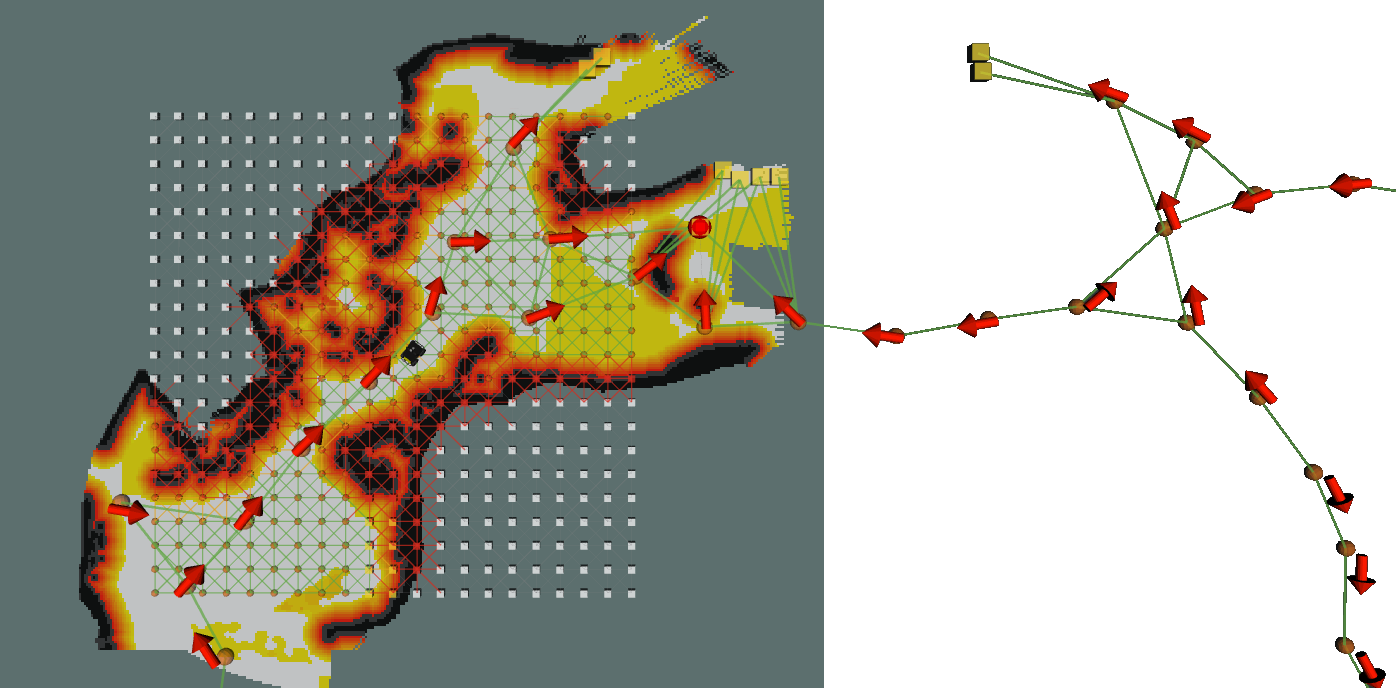
\includegraphics[width=.8\columnwidth]{figures/QMDP_Policy.png}
  \caption{QMDP policy (red arrows displayed above \textit{breadcrumb} nodes) for Global Coverage Planning (GCP). A red sphere indicates the QMDP frontier goal.}
  \label{fig:graph-level-planner}
\end{figure}


\begin{figure*}[h!]
\centering
    \begin{tikzpicture}
	    \node[anchor=south west,inner sep=0] (image) at (0,0) {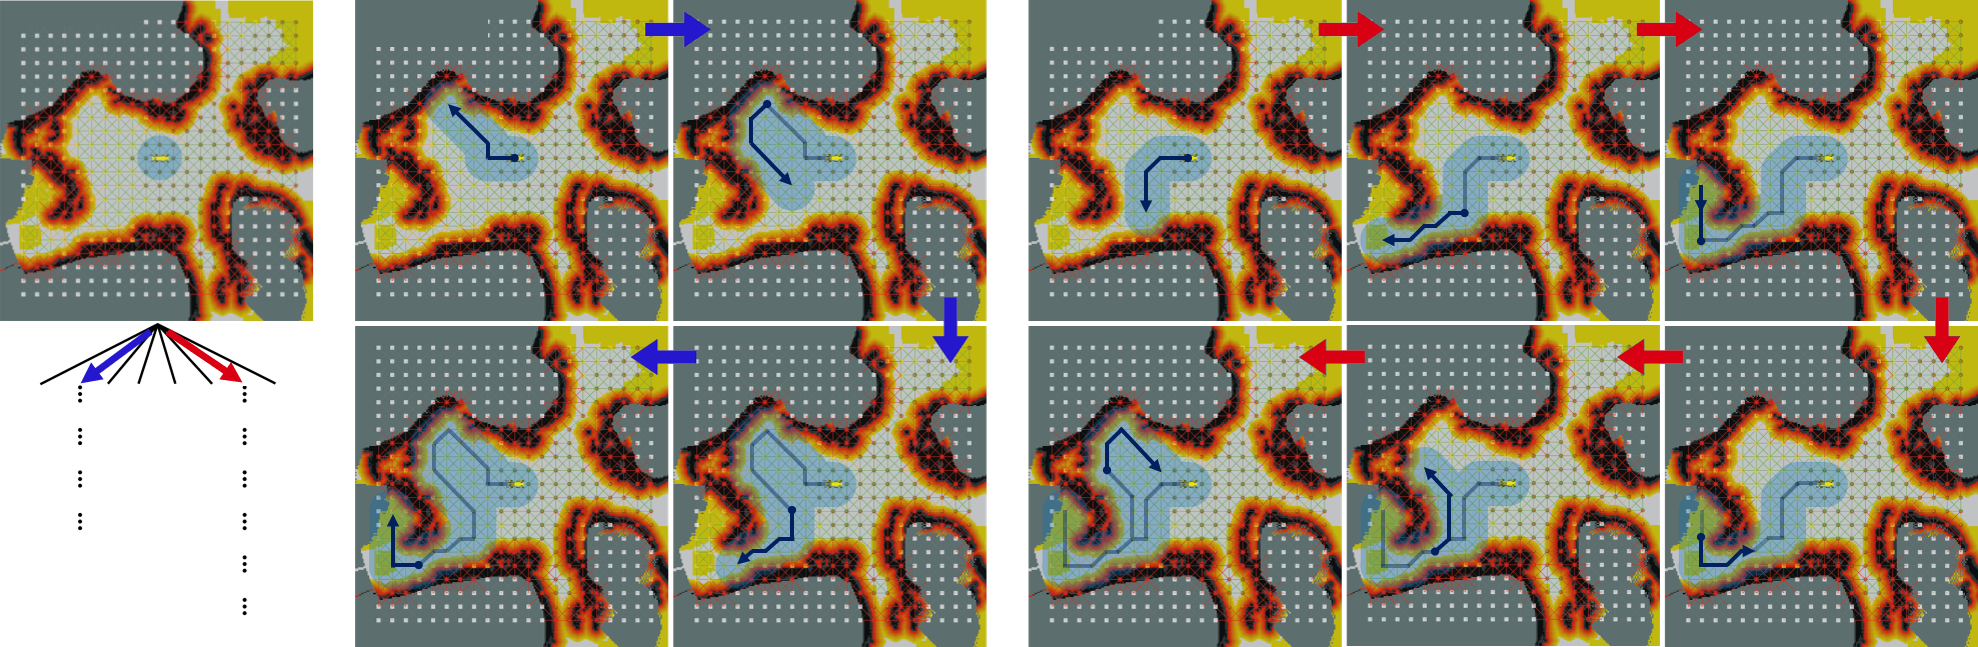
\includegraphics[width=1\textwidth]{figures/tree_figure_v9_ppt_v4}};
	    \begin{scope}[x={(image.south east)},y={(image.north west)}]
	    
    	    % Annotations [Big Labels]
	        \definecolor{mycolor_red}{RGB}{195.2, 0.0, 19.8}
	        \definecolor{mycolor_blue}{RGB}{37.2, 24, 204.6}
	        \node [above left,align=right,color=mycolor_blue] at (0.25,0.92) {Path $A$};
	        \node [above left,align=right,color=mycolor_red] at (0.59,0.92) {Path $B$};
	        \node [font=\scriptsize, above left,align=right,black] at (0.078,0.935) {Initial State};
	        
    	    % Annotations [W0]
	    	\node [font=\fontsize{4pt}{0}, above left,align=right,black] at (0.07,0.49) {$(W_0,Q_0)$};
	    	
    	    % Annotations [Tree]
	    	\node [font=\fontsize{4pt}{0}, above left,align=right,black] at (0.085,0.33) {$(W_{1a},Q_{1a})$};
	    	\node [font=\fontsize{4pt}{0}, above left,align=right,black] at (0.085,0.265) {$(W_{2a},Q_{2a})$};
	    	\node [font=\fontsize{4pt}{0}, above left,align=right,black] at (0.085,0.20) {$(W_{3a},Q_{3a})$};
	   % 	\node [font=\fontsize{4pt}{0}, above left,align=right,black] at (0.085,0.13) {$(W_{4a},Q_{4a})$};
	    	\node [font=\fontsize{4pt}{0}, above left,align=right,black] at (0.0755,0.13) {$(W_{1},Q_{1})$};
	    	
	    	\node [font=\fontsize{4pt}{0}, above left,align=right,black] at (0.166,0.33) {$(W_{1b},Q_{1b})$};
	    	\node [font=\fontsize{4pt}{0}, above left,align=right,black] at (0.166,0.265) {$(W_{2b},Q_{2b})$};
	    	\node [font=\fontsize{4pt}{0}, above left,align=right,black] at (0.166,0.20) {$(W_{3b},Q_{3b})$};
	    	\node [font=\fontsize{4pt}{0}, above left,align=right,black] at (0.166,0.13) {$(W_{4b},Q_{4b})$};
	    	\node [font=\fontsize{4pt}{0}, above left,align=right,black] at (0.166,0.067) {$(W_{5b},Q_{5b})$};
	   % 	\node [font=\fontsize{4pt}{0}, above left,align=right,black] at (0.166,0.00) {$(W_{6b},Q_{6b})$};
	    	\node [font=\fontsize{4pt}{0}, above left,align=right,black] at (0.16,0.00) {$(W_{1},Q_{1})$};
	    	
	    	% Annotations [Top]
	    	\node [font=\fontsize{4pt}{0}, above left,align=right,black] at (0.26,0.49) {$(W_{1a},Q_{1a})$};
	    	\node [font=\fontsize{4pt}{0}, above left,align=right,black] at (0.423,0.49) {$(W_{2a},Q_{2a})$};
	    	\node [font=\fontsize{4pt}{0}, above left,align=right,black] at (0.6,0.49) {$(W_{1b},Q_{1b})$};
	    	\node [font=\fontsize{4pt}{0}, above left,align=right,black] at (0.76,0.49) {$(W_{2b},Q_{2b})$};
	    	\node [font=\fontsize{4pt}{0}, above left,align=right,black] at (0.92,0.49) {$(W_{3b},Q_{3b})$};
	    	
	    	% Annotations [Bottom]
	   % 	\node [font=\fontsize{4pt}{0}, above left,align=right,black] at (0.26,-0.01) {$(W_{4a},Q_{4a})$};
	    	\node [font=\fontsize{4pt}{0}, above left,align=right,black] at (0.25,-0.01) {$(W_{1},Q_{1})$};
	    	\node [font=\fontsize{4pt}{0}, above left,align=right,black] at (0.423,-0.01) {$(W_{3a},Q_{3a})$};
	    	\node [font=\fontsize{4pt}{0}, above left,align=right,black] at (0.59,-0.01) {$(W_{1},Q_{1})$};
	    	\node [font=\fontsize{4pt}{0}, above left,align=right,black] at (0.76,-0.01) {$(W_{5b},Q_{5b})$};
	    	\node [font=\fontsize{4pt}{0}, above left,align=right,black] at (0.92,-0.01) {$(W_{4b},Q_{4b})$};
	    \end{scope}
	\end{tikzpicture}	
  \caption{Toy example of coverage path planning on the Local IRM with Monte-Carlo Tree Search. Robot field-of-view is represented by blue circle. The state contains the coverage state of the environment, $W$, and the robot state, $Q$. Macro actions (6 steps on Local IRM) associated with two tree branches (paths \textit{A} and \textit{B}) are shown. Note that the final states in each branch are identical. Path \textit{A} is evaluated to be more rewarding than \textit{B} since fewer actions were required to cover the same area.}
  \label{fig:lattice-level-planner}
\end{figure*}








\phdone{GCP Functionality}
In our cascaded hierarchical optimization framework, we first solve for the global policy in Eq.~(\ref{eq:glp_optimization}).
As mentioned in Section~\ref{ssec:hierarchical_policy}, the outcome of the global policy is a parameter for the local policy.
This means that Global Coverage Planner (GCP) for Eq.~(\ref{eq:glp_optimization}) provides \textit{global guidance} to Local Coverage Planner (LCP) for Eq.~(\ref{eq:llp_optimization}).
The global guidance is for the coverage performance and completeness in a global sense, and especially helpful when there is no local area for LCP to cover.

\phdone{GCP Problem Characteristics--Large-scale}
There are special characteristics to note in global coverage planning. 
First, the environment size can be very large (> 1~km), so GCP should be able to reason over more than hundreds of nodes on the Global IRM.
%
%
\phdone{GCP Problem Characteristics--Frontiers as terminal nodes}
Second, as the role of GCP is to guide the robot to an uncovered area and let LCP lead the local coverage behavior, GCP's policy search can terminate at frontier nodes on the Global IRM.
%
%
\phdone{GCP Problem Approximation}
Note that the second characteristic can help to mitigate the challenge from the first characteristic.
By considering the frontier nodes as terminal nodes in the belief space, we can assume no changes to be made to the world coverage state before the termination, and thus, we can omit $W$ from the state space for GCP.
Then, we can utilize simple and efficient POMDP solvers for a long horizon planning.


\phdone{POMDP Solver for GCP}
In this work, we adopt the QMDP approach for the global coverage planning \cite{littman1995learning}.
The key idea of QMDP is to assume the state becomes fully observable after one step of action, so that the value function for further actions can be evaluated efficiently in an MDP (Markov Decision Process) setting.
In our global coverage planning domain, we can consider the first step of action is for the robot to snap to one of the nearby node in Global IRM, and then, the robot pose is assumed to be fully observable, while the world occupancy and coverage states remain constant.


\phdone{QMDP Details}
More formally, we solve for $Q^g_{\mathrm{MDP}}(s^g, a^g)$ by ignoring uncertainty in robot pose $q^g$ and the change of $\hat{W}^g_{cov}$, where $s^g \in N^g$ and $a^g$ is a control to move to a neighbor node $s'^g \in N^g$.
In this MDP setting, $Q^g_{\mathrm{MDP}}(s^g, a^g)$ can be learned by Value Iteration very efficiently even for a long discount horizon.
%
Then, we can evaluate the Q-function in Eq.~(\ref{eq:q_function}) in a POMDP setting for the current belief and the feasible one-step actions, i.e.,
$Q(b^g, a^g) = \int_{s^g} b(s^g) Q^g_{\mathrm{MDP}}(s^g, a^g) \mathrm{d}s^g$.
%
Finally, a POMDP policy can be obtained as follows:
$\pi^g(b^g) = \argmax_{a^g \in \mathbb{A}^g} Q(b^g, a^g)$.
%
An example of the GCP policy is depicted in Fig.~\ref{fig:graph-level-planner}.
% [TODO] See Algorithm~\ref{alg:PLGRIM} for more details.



%% MANUALLY NUMBERED!
\subsubsection{4.3.2. Local Coverage Planner} \label{sssec:LCP}
\phdone{LCP Functionality}
In the hierarchical optimization framework, Local Coverage Planner (LCP) is who solves Eq.~(\ref{eq:llp_optimization}), given a parameter input from Global Coverage Planner (GCP).
LCP constructs a high-fidelity policy by considering the information gathering (with visibility check given obstacles), traversal risk (based on proximity to obstacles, terrain roughness, and slopes), and robot's mobility constraints (such as acceleration limits and non-holonomic constraints of wheeled robots).


\phdone{LCP Problem Characteristics}
% LCP has multiple operation modes based on the parameter input $\theta^\ell \in \Theta^\ell = \mathbb{A}^g$ from GCP,
LCP has multiple operation modes based on the parameter input $\theta^\ell = a^g \in \mathbb{A}^g$ from GCP,
where the target frontier node in Global IRM, $\hat{w}^g_f \in N^g$, can be extracted from the given global-level control $a^g$.
%
If $\hat{w}^g_f$ is within the Local IRM range, i.e., $\hat{w}^g_f \in \hat{W}^\ell$, then LCP performs the normal optimization as described in Eq.~(\ref{eq:llp_optimization}) for the local coverage behaviors.
If $\hat{w}^g_f \notin \hat{W}^\ell$, LCP simply instantiates a high-fidelity control of the given global-level control $a^g$ to follow the guidance of GCP.



\phdone{POMDP Solver LCP}
In order to solve Eq.~(\ref{eq:llp_optimization}) we employ POMCP (Partially Observable Monte Carlo Planning) algorithm \cite{silver2010monte}.
POMCP is a widely-adopted POMDP solver that leverages the Monte Carlo sampling technique to alleviate both of the curse of dimensionality and history.
Given a generative model (or a black box simulator) for discrete action and observation spaces, POMCP can learn the value function of near-optimally reachable belief space with adequate exploration-exploitation trade-off.


\phdone{POMCP Details}
More concretely, POMCP evaluates $Q^\ell(b^\ell, a^\ell)$ in Eq.~(\ref{eq:q_function}) by unrolling the recursive value backpropagation, with a set of sampled action-observation sequences.
% [TODO] Provide a more concrete example with formulation.
UCT algorithm for action selection helps to balance between exploration and exploitation to learn the Q-values.
Initially it explored the search space (possible action-observation sequences) with a random or heuristically guided rollout policy.
While incrementally building the belief tree it gradually exploits the learned values for more focused exploration with likely-optimal action-observation sequences (i.e., more focused exploration of the likely-reachable subspace by the optimal policy).
See illustration of local coverage planning in Fig.~\ref{fig:lattice-level-planner}.




\subsection{Resilient Receding Horizon Planning} \label{ssec:resilient_rhp}

\phdone{Consistency and Resiliency}
We extend the receding-horizon \textit{local} cover planning problem
in Eq.~(\ref{eq:llp_optimization}) to address the challenge between plan consistency and resiliency, described in Section~\ref{ssec:challenges}:
\textit{consistency} over consecutive plans to avoid unnecessary rotations, slow-down, or back-and-forth motions,
and \textit{resiliency} in a new plan in the presence of unforeseen hazard or anomalies.
% Consistency is related to how conformable the beginning of the new policy is to the end of the previous policy, while resiliency is related to 
In normal operations, consistency is preferred so that the robot can move effectively and make greater mission progress, while in abnormal situations, resiliency is required to ensure to the robot's safety and adapt to the unexpected changes.


\phdone{Receding Horizon Planning Re-formulation}
Let us consider the optimization problem in Eq.~(\ref{eq:llp_optimization}) but given the previous planning episode policy, i.e., 
$\pi_{t:t+T}^*(b; \pi_{t-\Delta t:t+T-\Delta t}^-)$, where $\pi_{t-\Delta t:t+T-\Delta t}^-$ is the previous policy constructed at time $(t - \Delta t)$ for a finite horizon with a length of $T$.
% $\pi_{t:t+T}^*(b; \pi_{t-\Delta t:t+T-\Delta t}^-) = \argmax_{\pi \in \Pi_{t:t+T}} \, \mathbb{E} \sum_{t'=t}^{t+T} \gamma^{t'-t} r(b_{t'}, \pi(b_{t'}; \pi_{t-\Delta t:t+T-\Delta t}^-))$.
%
% % \begin{align}
% %   \pi_{t:t+T}^*(b) &= \argmax_{\pi \in \Pi_{t:t+T}} \, \mathbb{E} \sum_{t'=t}^{t+T} \gamma^{t'-t} r(b_{t'}, \pi(b_{t'})),
% % \end{align}
% \begin{align}
%   &\pi_{t:t+T}^*(b; \pi_{t-\Delta t:t+T-\Delta t}^-) 
%   \nonumber \\
%   &= \argmax_{\pi \in \Pi_{t:t+T}} \, \mathbb{E} \sum_{t'=t}^{t+T} \gamma^{t'-t} r(b_{t'}, \pi(b_{t'}; \pi_{t-\Delta t:t+T-\Delta t}^-)),
%   \label{eq:revised_receding_objective_function}
% \end{align}
%
% We define an optimization variable $\tau_t$ that controls how much the new policy should observe the previous policy for the consistency 
We define another optimization variable $\tau_t$ that specifies how long the new policy should observe the previous policy.
A larger $\tau_t$ will enforce the consistency, while a smaller $\tau_t$ will enhance the resiliency.

% Here we consider a joint optimization problem how much of the previous policy should be preserved as follows:
% \begin{align}
%   % &\left(\pi_{t:t+T}^*(b; \pi_{{t'}-\Delta t:{t'}-\Delta t+T}^*), \, \tau_t^*\right)
%   % &\left(\pi_{t:t+T}^*, \, \tau_t^*\right)
%   &(\pi_{t:t+T}^*, \, \tau_t^*)
%   \nonumber \\
%   & = \argmax_{\pi \in \Pi_{t:t+T}, \, \tau \in [0, T-\Delta t]} \, \mathbb{E} \sum_{t'=t}^{t+\tau} \gamma^{t'-t} r(b_{t'}, \pi(b_{t'}; \pi_{{t'}-\Delta t:{t'}+T-\Delta t}^-))
%   \nonumber \\
%   &\quad + \sum_{t'=t+\tau}^{t+T} \gamma^{t'-t} r(b_{t'}, \pi(b_{t'}))
%   % \\
%   % & = \argmax_{\pi \in \Pi_{t:t+T}, \, \tau \in [0, T-\Delta t]} \, \mathbb{E} \sum_{t'=t}^{t+\tau} \gamma^{t'-t} r(b_{t'}, \pi_{{t'}-\Delta t:{t'}+T-\Delta t}^-(b_{t'}))
%   % \nonumber \\
%   % &\quad + \sum_{t'=t+\tau}^{t+T} \gamma^{t'-t-\tau} r(b_{t'}, \pi(b_{t'})),
% \end{align}

A joint optimization problem for $\pi_{t:t+T}^*$ and $\tau_t^*$ for a planning episode at time $t$ can be described as follows:
% \begin{align}
%   &(\pi_{t:t+T}^*, \, \tau_t^*) = \argmax_{\pi \in \Pi_{t:t+T}, \, \tau \in [0, T-\Delta t]}
%   \nonumber \\
%   &  \, \mathbb{E} \sum_{t'=t}^{t+\tau} \gamma^{t'-t} r(b_{t'}, \pi(b_{t'}; \pi_{{t'}-\Delta t:{t'}+T-\Delta t}^-))
%   \nonumber \\
%   &\quad + \sum_{t'=t+\tau}^{t+T} \gamma^{t'-t} r(b_{t'}, \pi(b_{t'}))
% \end{align}
%
% \begin{align}
%   &(\pi_{t:t+T}^*, \, \tau_t^*)
%   \nonumber \\
%   & = \argmax_{\pi \in \Pi_{t:t+T}, \, \tau \in [0, T-\Delta t]} \, \mathbb{E} \sum_{t'=t}^{t+\tau} \gamma^{t'-t} r(b_{t'}, \pi(b_{t'}; \pi_{{t'}-\Delta t:{t'}+T-\Delta t}^-))
%   \nonumber \\
%   &\quad + \sum_{t'=t+\tau}^{t+T} \gamma^{t'-t} r(b_{t'}, \pi(b_{t'}))
% \end{align}
%
% \begin{align}
%   &(\pi_{t:t+T}^*, \, \tau_t^*)%   \nonumber \\
%   & = \argmax_{\pi \in \Pi_{t:t+T}, \, \tau \in [0, T-\Delta t]} \, \mathbb{E} \Biggl[ \sum_{t'=t+\tau}^{t+T} \gamma^{t'-t} r(b_{t'}, \pi(b_{t'}))
%   \nonumber \\
%   &\quad + \sum_{t'=t}^{t+\tau} \gamma^{t'-t} r(b_{t'}, \pi(b_{t'}; \pi_{{t'}-\Delta t:{t'}+T-\Delta t}^-)) \Biggr]
% \end{align}
\begin{align}
  &(\pi_{t:t+T}^*, \, \tau_t^*)
  \nonumber \\
  & = \argmax_{\pi \in \Pi_{t:t+T}, \, \tau \in [0,\, T-\Delta t]} \, \mathbb{E} \left[ \sum_{t'=t+\tau}^{t+T} \gamma^{t'-t} r(b_{t'}, \pi(b_{t'})) \right.
  \nonumber \\
  &\quad \left. + \sum_{t'=t}^{t+\tau} \gamma^{t'-t} r(b_{t'}, \pi(b_{t'}; \pi_{{t'}-\Delta t:{t'}+T-\Delta t}^-)) \right] \!\!.
  \label{eq:resiliency_optimization}
\end{align}
\normalsize
%
As an approximate but efficient way of solving Eq.~(\ref{eq:resiliency_optimization}), we first solve for $\tau^*_t$ and then $\pi^*_{t+\tau^*_t:t+T}$ accordingly, i.e., 
% \begin{align}
%   & \pi_{t+\tau^*_t:t+T}^* = \argmax_{\pi \in \Pi_{t+\tau^*_t:t+T}} \, \mathbb{E} \sum_{t'=t+\tau^*_t}^{t+T} \gamma^{t'-t-\tau^*_t} r(b_{t'}, \pi(b_{t'})),
%   \label{eq:resiliency_pi}
%   \\
%   &\text{where}
%   \nonumber \\
%   & \tau^*_t = \argmax_{\tau \in [0,\, T-\Delta t]} \mathbb{E} \sum_{t'=t}^{t+\tau} \gamma^{t'-t} r(b_{t'}, \pi_{{t'}-\Delta t:{t'}+T-\Delta t}^-(b_{t'})).
%   \label{eq:resiliency_tau}
% \end{align}
%
%
% \begin{align}
%   & \tau^*_t = \argmax_{\tau \in [0,\, T-\Delta t]} \mathbb{E} \sum_{t'=t}^{t+\tau} \gamma^{t'-t} r(b_{t'}, \pi_{{t'}-\Delta t:{t'}+T-\Delta t}^-(b_{t'})),
%   \label{eq:resiliency_tau}
%   \\
%   & \pi_{t+\tau^*_t:t+T}^* = \argmax_{\pi \in \Pi_{t+\tau^*_t:t+T}} \, \mathbb{E} \sum_{t'=t+\tau^*_t}^{t+T} \gamma^{t'-t-\tau^*_t} r(b_{t'}, \pi(b_{t'})).
%   \label{eq:resiliency_pi}
% \end{align}
%
\begin{align}
  & \pi_{t+\tau^*_t:t+T}^* = \argmax_{\pi \in \Pi_{t+\tau^*_t:t+T}} \, \mathbb{E} \sum_{t'=t+\tau^*_t}^{t+T} \gamma^{t'-t-\tau^*_t} r(b_{t'}, \pi(b_{t'})),
  \label{eq:resiliency_pi}
  \\
  &\text{where}
  \nonumber \\
  & \tau^*_t = \argmax_{\tau \in [0,\, T-\Delta t]} \mathbb{E} \sum_{t'=t}^{t+\tau} \gamma^{t'-t} r(b_{t'}, \pi_{{t'}-\Delta t:{t'}+T-\Delta t}^-(b_{t'})).
  \label{eq:resiliency_tau}
\end{align}
\normalsize
%
Note that Eq.~(\ref{eq:resiliency_tau}) is now independent of $\pi_{t:t+T}^*$ by reusing $\pi_{{t'}-\Delta t:{t'}+T-\Delta t}^-$ from time $t$ to $t + \tau$.
The evaluation of the accumulated rewards is based on the updated belief (e.g., updated $W_{occ}$ given new range sensor readings), so that $\tau^*_t$ can be determined based on the disagreement (e.g., high traversal risk) of the previous policy with the updated robot-world belief.

Given $\tau^*_t$, Eq.~(\ref{eq:resiliency_pi}) becomes identical to Eq.~(\ref{eq:llp_optimization}) except for the change in the start time,
and can be solved by LCP described in Section~\ref{sssec:LCP}.2.  % HACK: MANUALLY NUMBERED!
%
The final receding horizon policy can be constructed by concatenating the previous and a new policies as $\pi_{t:t+T}^* = [\pi_{t:t+\tau^*_t}^-; \, \pi_{t+\tau^*_t:t+T}^*]$.




\begin{figure}
	\centering
	%  	\subfloat[Simulated \\Cave]{
	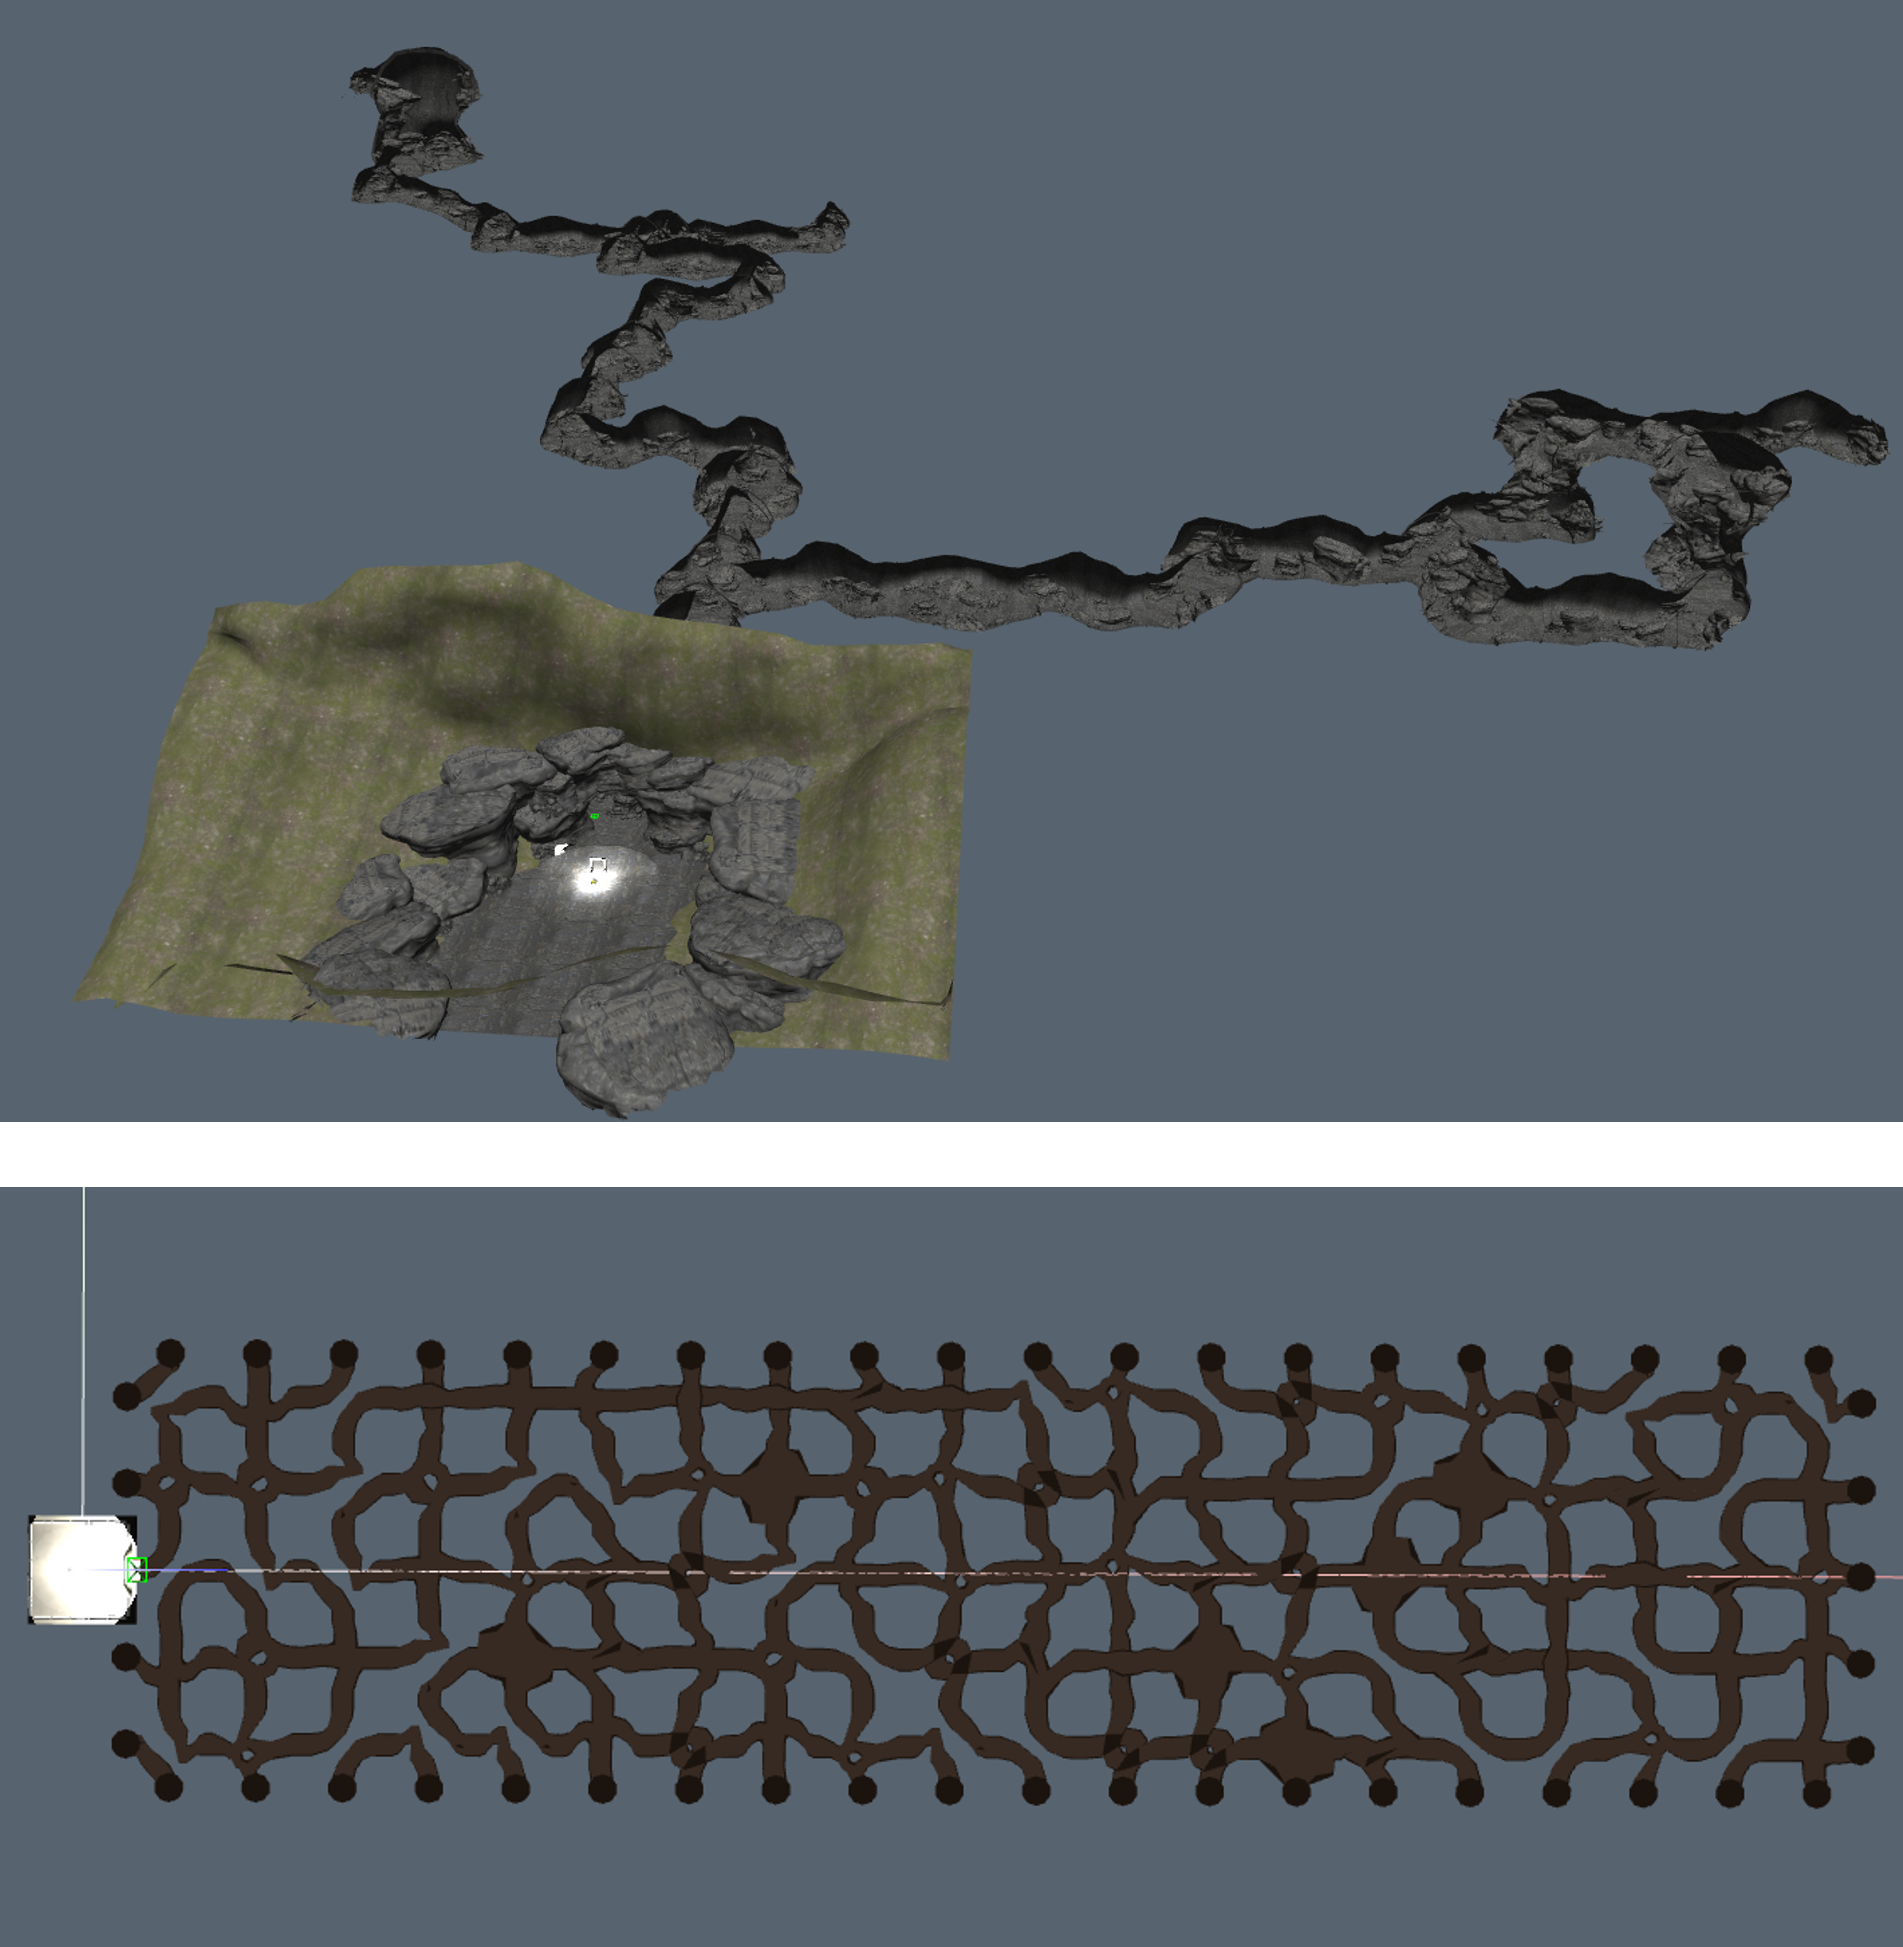
\includegraphics[width=0.63\columnwidth]{figures/together.png}
	%  	}
	% %  	\quad
	% 	\subfloat[Simulated \\Maze]{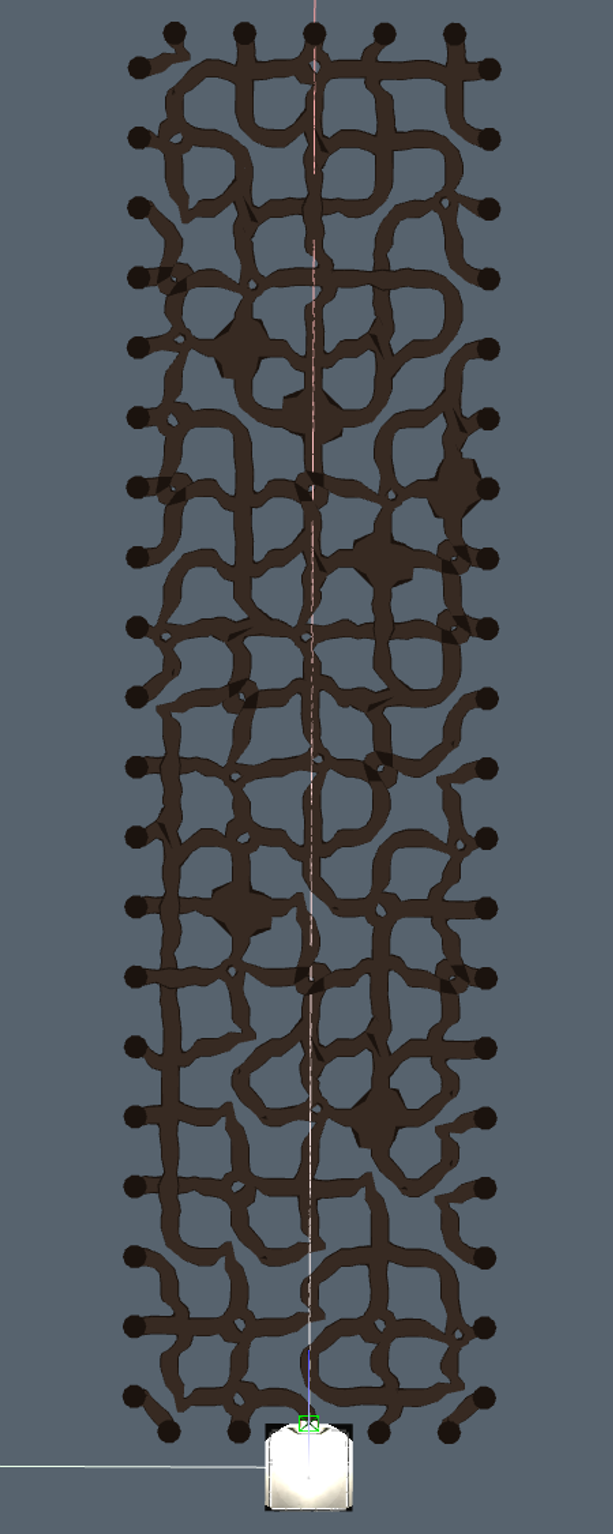
\includegraphics[width=0.3\columnwidth, angle=90]{IRM_Planning/figures/maze.png}}
	\caption{Simulated cave (top) and maze (bottom).}
	\label{fig:maps_of_cave}
\end{figure}



\section{Experimental Results}\label{sec:exp_results}
%\ph{Intro}
In order to evaluate our proposed framework, we performed high-fidelity simulation studies with a four-wheeled vehicle (Husky robot) and real-world experiments with a quadruped (Boston Dynamics Spot robot). Both robots are equipped with custom sensing and computing systems~\cite{AutoSpot}, enabling high levels of autonomy and communication capabilities~\cite{Otsu2020}. The entire autonomy stack runs in real-time on an Intel Core i7 processor with 32 GB of RAM. The stack relies on a multi-sensor fusion framework. The core of this framework is 3D point cloud data provided by LiDAR range sensors mounted on the robots~\cite{Ebadi2020}.


\subsection{Baseline Algorithms}
We compared our PLGRIM framework against a competitive local coverage planner (next-best-view scheme) and a competitive global coverage planner (frontier-based scheme). 
\vspace{-4pt}
\begin{enumerate}[label={\arabic*)}]
  \itemsep0em 
  \setlength{\itemsep}{0pt}
  \setlength{\parskip}{0pt}
  \item \textbf{Local IRM-based Next-Best-View (NBV)}:
  NBV is a widely-adopted local coverage planner that returns a path to the best next view point to move to.
	It uses an information gain-based reward function as ours but limits the policy search space to a set of shortest paths to sampled view points around the robot.
  While its policy is with a high spatial resolution, it depends on a lower-level deterministic path planner to get a path to each view point, and therefore it cannot consider probabilistic risks or information gathering when finding a path to the view points.
  \item \textbf{Hierarchical Frontier-based Exploration (HFE)}:
	Frontier-based exploration is a prevalent global coverage planning approach that interleaves moving to a frontier node and creating new frontiers until there are no more frontiers left.
	It can ensure the global completeness of exploration but often suffers from the local suboptimality due to its large scale of the policy space and myopic one-step look-ahead decision making.
	HFE is an extended version of frontier-based approach that mitigates such problems by limiting the scope of frontier selection to a local area as long as there are any frontiers near to the robot.
	However, it is still subject to the inherited suboptimality because of the low spatial resolution of its policy.
\end{enumerate}
\vspace{-4pt}
Note that in order to achieve reasonable performance in the complex simulated environments we allowed each baselines to leverage our Local/Global IRM construction modules described in Section~\ref{ssec:belief-managers}.


\begin{figure*}[t!]
    \centering
     	\subfloat[Subway 1x]{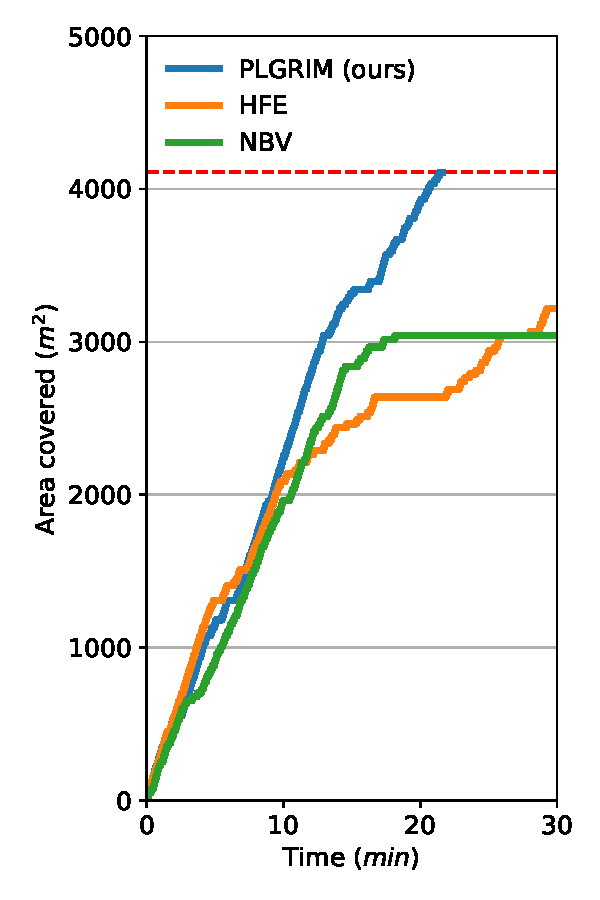
\includegraphics[width=0.392\columnwidth]{figures/areacov_plots/subway1x.pdf}}
    	\subfloat[Subway 2x]{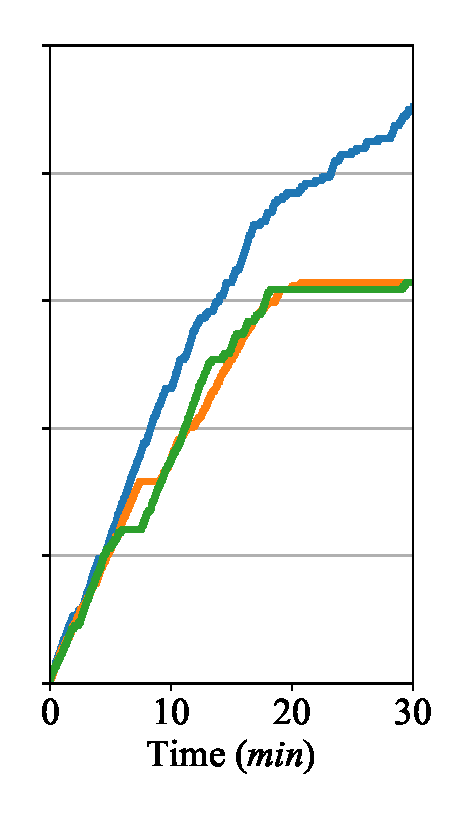
\includegraphics[width=0.31\columnwidth]{figures/areacov_plots/subway2x.pdf}}	
    	\subfloat[Subway 3x]{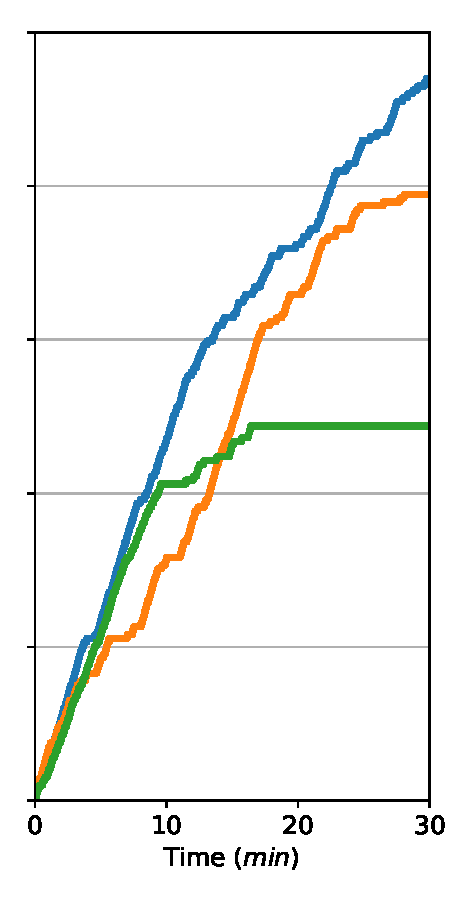
\includegraphics[width=0.31\columnwidth]{figures/areacov_plots/subway3x.pdf}}	
      \subfloat[][Simulated \\Cave]{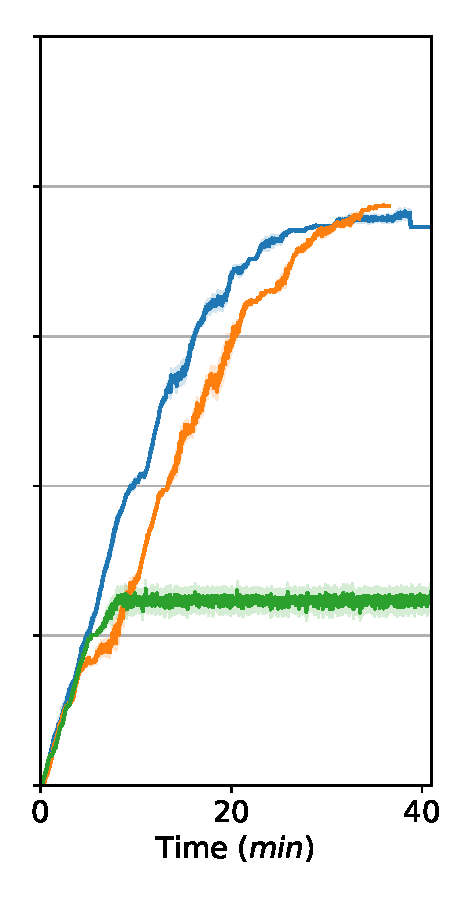
\includegraphics[width=0.31\columnwidth]{figures/areacov_plots/comparison_simple_cave.pdf}}
      \subfloat[][Simulated \\Maze]{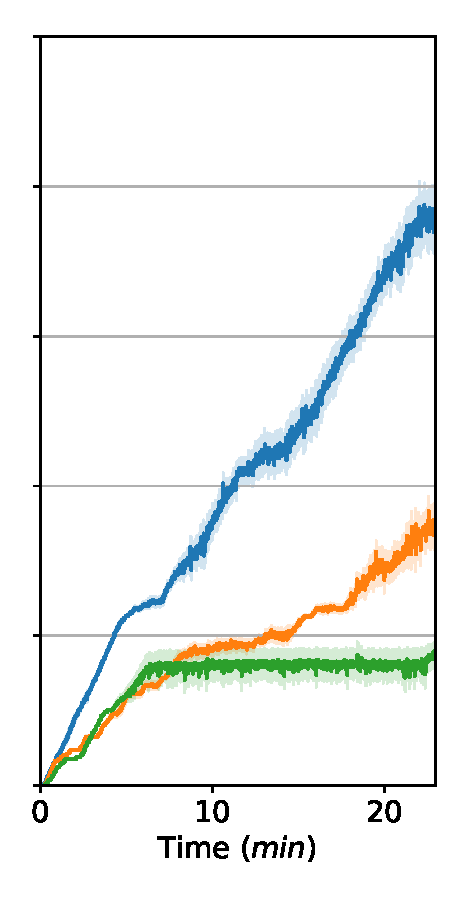
\includegraphics[width=0.31\columnwidth]{figures/areacov_plots/comparison_cave_cropped.pdf}}
    	\subfloat[Lava Tube]{%
        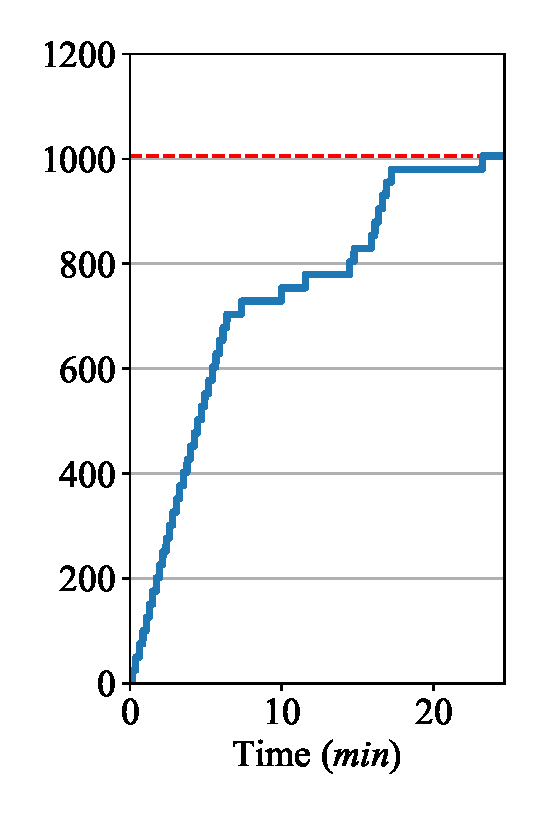
\includegraphics[clip,width=0.34\columnwidth]{figures/areacov_plots/lava_tube.pdf}%
        }
				\caption{Exploration by PLGRIM and baseline methods in simulated subway environments of increasing size (a)-(c), and in simulated and real-world cave environments (d)-(f). For (d) and (e), the covered area is the average of two runs. Red dashed lines indicate 100\% coverage of the environments where applicable.}
    \label{fig:all_together_plot}
\end{figure*}



\subsection{Test Environments}

\vspace{0pt}
\begin{enumerate}[label={\arabic*)}]
  \itemsep0em 
  \setlength{\itemsep}{0pt}
  \setlength{\parskip}{0pt}
  \item \textbf{Simulated Subway Station}: Large interconnected, polygonal rooms with level-floors, which are free of obstacles.
  \item \textbf{Simulated Cave \& Maze}: Unstructured environments with complex terrain (e.g. rocks, steep slopes) and topology, including narrow passages, dead-ends, open-spaces, and branches with fluctuating curvature. 
  \item \textbf{Lava Tube Cave}: Located in Lava Beds National Monument, Tulelake, CA. The cave consists of a main lava tube and a series of smaller, auxiliary tubes branching off. The floor is composed of undulating smooth and ropy masses of cooled lava. Some areas of the floor are covered by large boulders, due to ceiling breakdown.
\end{enumerate}
\vspace{-4pt}


\subsection{Simulation Results}


Fig.~\ref{fig:all_together_plot}(a)-(c) shows the scalability of our proposed algorithm. 
In a relatively small environment without complex features (Subway 1x), NBV performance competitively as it evaluates high-resolution paths, considering the information gain.
However, as the scale grows, its myopic planning easily gets stuck and the robot's coverage rate significantly decreases. 
% Note that the ground truth environment information is not accessible by the robot.
HFE shows inconsistent performance in different environments.
Its global planning policy is simply depth-first frontier selection, so in such a wide-open environment its decision making often becomes suboptimal.
%

Fig.~\ref{fig:all_together_plot}(d)-(f) shows the coverage rate for the algorithms in the unstructured cave environments. 
HFE performs well in the simulated cave environment which has relatively simple topology, but works poorly in maze environment.
The frontier-based exploration has sparse action space, which is intrinsically brittle especially in narrow passages or sharp corners.
PGLRIM outperforms over these environments as well, thanks to its dense local coverage planning and large-scale global guidance.

\begin{figure*}[h!]
\centering
    \begin{tikzpicture}
	    \node[anchor=south west,inner sep=0] (image) at (0,0) {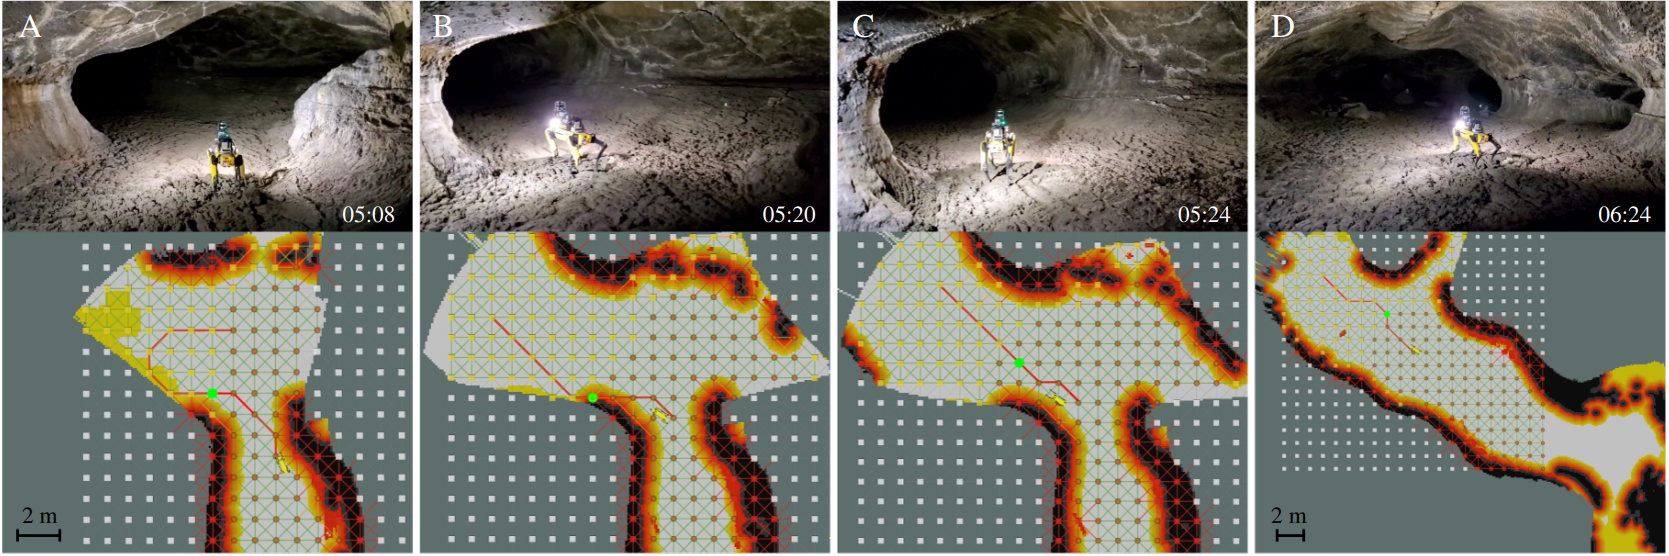
\includegraphics[width=.75\textwidth]{figures/MLP_screenshot.png}};
	\end{tikzpicture}		
\caption{LCP plans looping path that fully covers area represented by Local IRM (snapshot A). Path is updated to extend towards large uncovered swath while maintaining consistency with prior path. Risk map update reveals that path has entered a hazardous area---wall of lava tube (snapshot B). As a demonstration of LCP's resilience, path shifts away from hazardous area and robot is re-directed towards center of tube (snapshot C). One minute later, robot encounters fork in cave system. LCP path curves slightly toward fork apex before entering larger, less-risky channel (snapshot D). } \label{fig:mlp_hardware_tests} 
\end{figure*}

\begin{figure*}[h!]
\centering
    \begin{tikzpicture}
	    \node[anchor=south west,inner sep=0] (image) at (0,0) {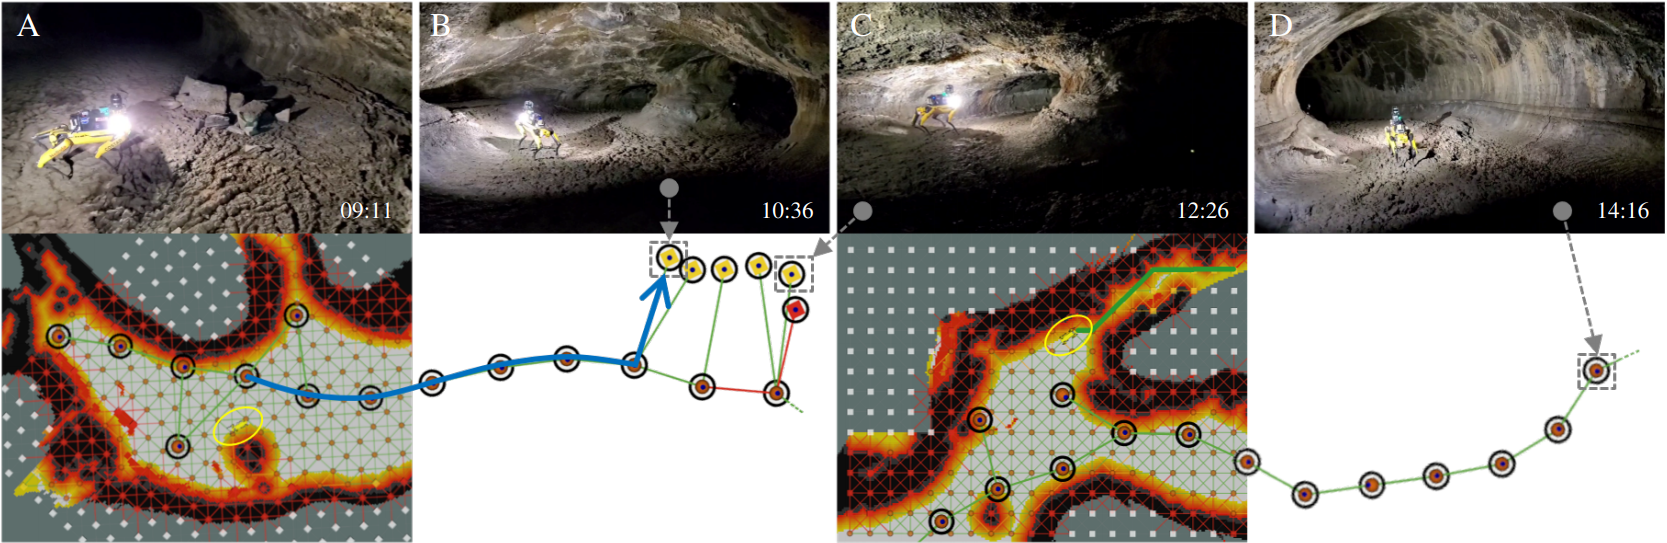
\includegraphics[width=0.75\textwidth]{figures/GLP_screenshot.png}};
	\end{tikzpicture}	
\caption{GCP plans path (blue) along Global IRM to frontier after local area is fully covered (snapshot A). Robot explores area around frontier (snapshot B), and then explores neighboring frontier at opening of side channel. LCP plans path (green) into channel (snapshot C). Later, after all local area has been explored, GCP guides robot back towards mouth of cave (snapshot D).} \label{fig:glp_hardware_tests} 
\end{figure*}



\begin{figure}
     \centering
  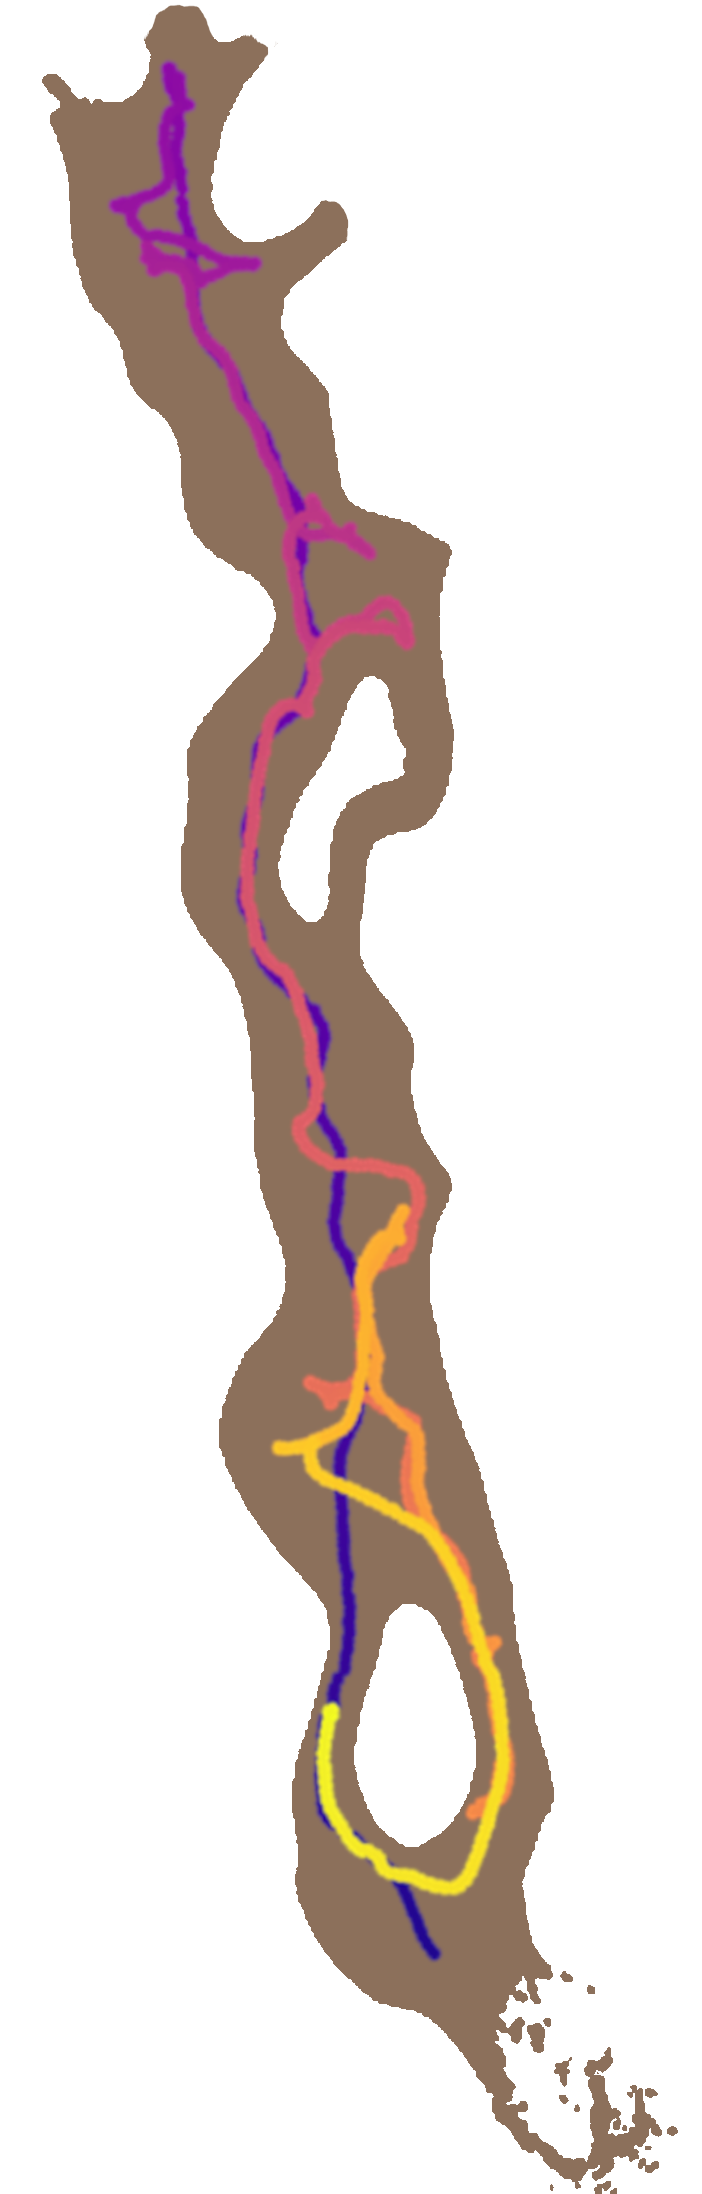
\includegraphics[width=0.45\columnwidth,angle=90, scale=0.7
  ]{figures/darpa_tv_test_figs/cave_path_overlay_lightbrown.png}%
	\caption{Robot trajectory on cave profile from hardware test.}
    \label{fig:lava_tube_traj}
\end{figure}


\subsection{Hardware Results}
We validated PLGRIM on a physical robot in a real-world environment. Fig.~\ref{fig:mlp_hardware_tests} and Fig.~\ref{fig:glp_hardware_tests} describe how the planner is able to overcome challenges posed by large-scale environments with difficult terrain. Namely, we address the \textit{Planner Horizon vs. Resolution} and \textit{Plan Consistency vs. Resiliency} challenges. Fig.~\ref{fig:lava_tube_traj} shows the trajectory overlaid onto the cave profile, and Fig.~\ref{fig:all_together_plot}(c) shows the area covered over time.



%%%%%%%%%%%%%%%%%%%%%%%%%%%%%%%%%%%%%%%%%%%%%%%%%%%%%%%%%%%%%%%%%%%%%%%%%%%%%%%%
\section{Conclusion}\label{sec:conclusion}

In this work, we have developed a hierarchical framework for exploring large-scale unknown environments in a POMDP setting. 
To obtain a tractable solution, we discretize the belief space into a robot and task-relevant graph structure. This simplifies the planning problem and reduces our search space for good policies.
The hierarchical planning framework and formalization of the unified optimal policy allows us to solve the coverage planning problem in large-scale environments.
We demonstrate these capabilities in high-fidelity dynamic simulation environments and in real-world tests in a natural cave.  

Future work includes learning-based methods for graph expansion information gain estimation, and a richer incorporation of risk and time into the graph planning framework.
Another interesting venue is the extension of this framework to the multi-robot coverage problems.


\section*{Acknowledgment}
The work is partially supported by the Jet Propulsion Laboratory, California Institute of Technology, under a contract with the National Aeronautics and Space Administration (80NM0018D0004), and Defense Advanced Research Projects Agency (DARPA).



%%%%%%%%%%%%%%%%%%%%%%%%%%%%%%%%%%%%%%%%%%%%%%%%%%%%%%%%%%%%%%%%%%%%%%%%%%%%%%%%
\bibliographystyle{aaai21}
\bibliography{references}  % .bib


\end{document}
